\pdfoutput=1


% \documentclass[sigconf,anonymous,table]{acmart} %review,10pt
\documentclass[sigconf,table]{acmart} %review,10pt


\settopmatter{printacmref=false, printccs=true, printfolios=true} % We want page numbers on submissions


% https://tex.stackexchange.com/questions/346292/remove-conference-information-from-acm-2017-sigconf-template
%\settopmatter{printacmref=false} % Removes citation information below abstract
\renewcommand\footnotetextcopyrightpermission[1]{} % removes footnote with conference information in first column
%https://tex.stackexchange.com/questions/17768/remove-running-head-in-amsart
%\pagestyle{empty} % removes running headers


\fancyhf{} % Remove fancy page headers
\fancyfoot[C]{\thepage}


% Set letter paper size:
%\setlength{\paperheight}{11in}
%\setlength{\paperwidth}{8.5in}
%\usepackage[
%  pass,% keep layout unchanged
%  % showframe,% show the layout
%]{geometry}
% \usepackage[table]{xcolor}  %rowcolors and rowcolor
\usepackage{xcolor}  %rowcolors and rowcolor
\usepackage{tabularx}
% to be able to draw some self-contained figs
\usepackage{tikz}
\usepackage{amsmath}
\usepackage{graphicx}
\usepackage{booktabs}
\usepackage{latexsym} % \Diamond
\usepackage{array}    % p{}
\usepackage{multirow}
%\usepackage{subfigure}
\usepackage{subcaption}
\usepackage{algorithm}
\usepackage[noend]{algpseudocode}
\usepackage[font={small,bf}]{caption}  % must before threeparttable
\usepackage{threeparttable}
\usepackage{paralist}   % compactitem
\usepackage{xspace}
\usepackage{color}
\usepackage{adjustbox}
% \usepackage{balance}
\usepackage{wasysym}
\usepackage{rotating}   % turn
\usepackage{listings}
% %\usepackage{flushend}  %TODO add in the future
\usepackage{tabu}
% \usepackage{amssymb}
\usepackage{pifont}
\usepackage{framed}
\usepackage[shortlabels]{enumitem}
% \usepackage{authblk}
\usepackage{makecell}
\usepackage{appendix}
\usepackage{soul}
\setenumerate[1]{itemsep=0pt,partopsep=0pt,parsep=\parskip,topsep=2pt}
\setitemize[1]{itemsep=0pt,partopsep=0pt,parsep=\parskip,topsep=2pt}
\setdescription{itemsep=0pt,partopsep=0pt,parsep=\parskip,topsep=2pt}

%\usepackage[hyphens]{url}  % old ACM
\usepackage{url}            % new ACM
\def\UrlBreaks{\do\/\do-} % Break long url
%\usepackage[pdfborder={0 0 0}, citecolor=blue, linkcolor=blue, urlcolor=black, colorlinks=true]{hyperref}
\usepackage{hyperref}
%\usepackage[draft]{hyperref}
\usepackage{flushend}

% %a fix for making tabu and threeparttable work together
% %http://tex.stackexchange.com/a/56524
\usepackage{xpatch}
\usepackage{graphics}
\usepackage[utf8]{inputenc}
\usepackage{cleveref}
\usepackage{circledsteps}
\crefname{section}{§}{§§}
\Crefname{section}{§}{§§}
\newtheorem{definition}{Definition}
\makeatletter
\chardef\TPT@@@asteriskcatcode=\catcode`*
\catcode`*=11
\xpatchcmd{\threeparttable}
  {\TPT@hookin{tabular}}
  {\TPT@hookin{tabular}\TPT@hookin{tabu}}
  {}{}
\catcode`*=\TPT@@@asteriskcatcode
\makeatother

\usepackage{tcolorbox}
\tcbuselibrary{breakable, skins}
\tcbset{%
  label begin/.style={label={#1}},%          just for symmetry
  label end/.style={after upper=\label{#1}}% new end label
}
\newtcolorbox[%
auto counter]{mybox}[2][]{%
  enhanced jigsaw,
  breakable,
  #1}


% Copyright
\setcopyright{none}
%\setcopyright{acmcopyright}
%\setcopyright{acmlicensed}
% \setcopyright{rightsretained}
%\setcopyright{usgov}
%\setcopyright{usgovmixed}
%\setcopyright{cagov}
%\setcopyright{cagovmixed}

% DOI
% \acmDOI{10.475/123_4}

% ISBN
% \acmISBN{123-4567-24-567/08/06}

%Conference
% \acmConference[CCS'24]{ACM CCS Conference}{November 2024}{Salt Lake City, US}
% \acmYear{2024}
%\copyrightyear{2016}

% \acmPrice{15.00}

% \acmBadgeL[http://ctuning.org/ae/ppopp2016.html]{ae-logo}
% \acmBadgeR[http://ctuning.org/ae/ppopp2016.html]{ae-logo}


% tune title
% \makeatletter
% \def\@maketitle{\newpage
 % \null
 % \setbox\@acmtitlebox\vbox{%
% \baselineskip 20pt
% \vskip 1.5em                   % Vertical space above title.
   % \begin{center}
    % {\ttlfnt \@title\par}       % Title set in 18pt Helvetica (Arial) bold size.
    % \vskip 0.3em                % Vertical space after title.
% %This should be the subtitle.
% {\subttlfnt \the\subtitletext\par}\vskip 1.25em%\fi
    % {\baselineskip 16pt\aufnt   % each author set in \12 pt Arial, in a
     % \lineskip .5em             % tabular environment
     % \begin{tabular}[t]{c}\@author
     % \end{tabular}\par}
    % \vskip 0.8em               % Vertical space after author.
   % \end{center}}
 % \dimen0=\ht\@acmtitlebox
% % \advance\dimen0 by -12.75pc\relax % comment by Marco Daniel
 % \unvbox\@acmtitlebox
 % \ifdim\dimen0<0.0pt\relax\vskip-\dimen0\fi}
% \makeatother


%https://tex.stackexchange.com/questions/374932/a-white-number-inside-a-black-circle
%\newcommand*\circled[1]{\tikz[baseline=(char.base)]{
%            \node[shape=circle,fill,inner sep=1pt] (char) {\textcolor{white}{#1}};}}


\usepackage[skip=7pt]{caption}
\newcommand{\distance}{3pt}
\setlength{\textfloatsep}{\distance}%set distance between figure/tables on the top/bottom with text
\setlength{\floatsep}{\distance}%set distance between figures or tables
\setlength{\intextsep}{\distance}%set distance between figures/tables in text with text
\setlength{\dbltextfloatsep}{\distance} %distance between a figure/table spanning both columns and the text;
\setlength{\dblfloatsep}{\distance} %distance between two figures/tables spanning both columns.

\def\method{\text MixMin~}
\def\methodnospace{\text MixMin}
\def\genmethod{$\mathbb{R}$\text Min~}
\def\genmethodnospace{ $\mathbb{R}$\text Min}


\begin{document}

\title{\tool: Detecting Various DeFi Price Manipulations with LLM Reasoning}

% \author{
% Anonymous Submission
% }

\author{Juantao Zhong}
\affiliation{%
 \institution{The Hong Kong University of Science and Technology}
  \city{Hong Kong SAR}
  \country{China}}
\email{jzhong012@e.ntu.edu.sg}

\author{Daoyuan Wu}
\authornote{Daoyuan Wu and Juantao Zhong are the co-first authors.}
\affiliation{%
  \institution{The Hong Kong University of Science and Technology}
  \city{Hong Kong SAR}
  \country{China}}
\email{daoyuan@cse.ust.hk}

\author{Ye Liu}
\authornote{Ye Liu is the corresponding author.}
\affiliation{%
  \institution{Singapore Management University}
  \city{Singapore}
  \country{Singapore}}
\email{yeliu@smu.edu.sg}

\author{Maoyi Xie}
\affiliation{%
 \institution{Nanyang Technological University}
  \city{Singapore}
  \country{Singapore}}
\email{maoyi001@e.ntu.edu.sg}

\author{Yang Liu}
\affiliation{%
 \institution{Nanyang Technological University}
  \city{Singapore}
  \country{Singapore}}
\email{yangliu@ntu.edu.sg}

\author{Yi Li}
\affiliation{%
 \institution{Nanyang Technological University}
  \city{Singapore}
  \country{Singapore}}
\email{yi_li@ntu.edu.sg}

\author{Ning Liu}
\affiliation{%
 \institution{City University of Hong Kong}
  \city{Hong Kong SAR}
  \country{China}}
\email{ninliu@cityu.edu.hk}


%%
%% By default, the full list of authors will be used in the page
%% headers. Often, this list is too long, and will overlap
%% other information printed in the page headers. This command allows
%% the author to define a more concise list
%% of authors' names for this purpose.
% \renewcommand{\shortauthors}{}


%%
%% The abstract is a short summary of the work to be presented in the
%% article.
\begin{abstract}  
Test time scaling is currently one of the most active research areas that shows promise after training time scaling has reached its limits.
Deep-thinking (DT) models are a class of recurrent models that can perform easy-to-hard generalization by assigning more compute to harder test samples.
However, due to their inability to determine the complexity of a test sample, DT models have to use a large amount of computation for both easy and hard test samples.
Excessive test time computation is wasteful and can cause the ``overthinking'' problem where more test time computation leads to worse results.
In this paper, we introduce a test time training method for determining the optimal amount of computation needed for each sample during test time.
We also propose Conv-LiGRU, a novel recurrent architecture for efficient and robust visual reasoning. 
Extensive experiments demonstrate that Conv-LiGRU is more stable than DT, effectively mitigates the ``overthinking'' phenomenon, and achieves superior accuracy.
\end{abstract}  


\maketitle


\section{Introduction}
\label{sec:introduction}
The business processes of organizations are experiencing ever-increasing complexity due to the large amount of data, high number of users, and high-tech devices involved \cite{martin2021pmopportunitieschallenges, beerepoot2023biggestbpmproblems}. This complexity may cause business processes to deviate from normal control flow due to unforeseen and disruptive anomalies \cite{adams2023proceddsriftdetection}. These control-flow anomalies manifest as unknown, skipped, and wrongly-ordered activities in the traces of event logs monitored from the execution of business processes \cite{ko2023adsystematicreview}. For the sake of clarity, let us consider an illustrative example of such anomalies. Figure \ref{FP_ANOMALIES} shows a so-called event log footprint, which captures the control flow relations of four activities of a hypothetical event log. In particular, this footprint captures the control-flow relations between activities \texttt{a}, \texttt{b}, \texttt{c} and \texttt{d}. These are the causal ($\rightarrow$) relation, concurrent ($\parallel$) relation, and other ($\#$) relations such as exclusivity or non-local dependency \cite{aalst2022pmhandbook}. In addition, on the right are six traces, of which five exhibit skipped, wrongly-ordered and unknown control-flow anomalies. For example, $\langle$\texttt{a b d}$\rangle$ has a skipped activity, which is \texttt{c}. Because of this skipped activity, the control-flow relation \texttt{b}$\,\#\,$\texttt{d} is violated, since \texttt{d} directly follows \texttt{b} in the anomalous trace.
\begin{figure}[!t]
\centering
\includegraphics[width=0.9\columnwidth]{images/FP_ANOMALIES.png}
\caption{An example event log footprint with six traces, of which five exhibit control-flow anomalies.}
\label{FP_ANOMALIES}
\end{figure}

\subsection{Control-flow anomaly detection}
Control-flow anomaly detection techniques aim to characterize the normal control flow from event logs and verify whether these deviations occur in new event logs \cite{ko2023adsystematicreview}. To develop control-flow anomaly detection techniques, \revision{process mining} has seen widespread adoption owing to process discovery and \revision{conformance checking}. On the one hand, process discovery is a set of algorithms that encode control-flow relations as a set of model elements and constraints according to a given modeling formalism \cite{aalst2022pmhandbook}; hereafter, we refer to the Petri net, a widespread modeling formalism. On the other hand, \revision{conformance checking} is an explainable set of algorithms that allows linking any deviations with the reference Petri net and providing the fitness measure, namely a measure of how much the Petri net fits the new event log \cite{aalst2022pmhandbook}. Many control-flow anomaly detection techniques based on \revision{conformance checking} (hereafter, \revision{conformance checking}-based techniques) use the fitness measure to determine whether an event log is anomalous \cite{bezerra2009pmad, bezerra2013adlogspais, myers2018icsadpm, pecchia2020applicationfailuresanalysispm}. 

The scientific literature also includes many \revision{conformance checking}-independent techniques for control-flow anomaly detection that combine specific types of trace encodings with machine/deep learning \cite{ko2023adsystematicreview, tavares2023pmtraceencoding}. Whereas these techniques are very effective, their explainability is challenging due to both the type of trace encoding employed and the machine/deep learning model used \cite{rawal2022trustworthyaiadvances,li2023explainablead}. Hence, in the following, we focus on the shortcomings of \revision{conformance checking}-based techniques to investigate whether it is possible to support the development of competitive control-flow anomaly detection techniques while maintaining the explainable nature of \revision{conformance checking}.
\begin{figure}[!t]
\centering
\includegraphics[width=\columnwidth]{images/HIGH_LEVEL_VIEW.png}
\caption{A high-level view of the proposed framework for combining \revision{process mining}-based feature extraction with dimensionality reduction for control-flow anomaly detection.}
\label{HIGH_LEVEL_VIEW}
\end{figure}

\subsection{Shortcomings of \revision{conformance checking}-based techniques}
Unfortunately, the detection effectiveness of \revision{conformance checking}-based techniques is affected by noisy data and low-quality Petri nets, which may be due to human errors in the modeling process or representational bias of process discovery algorithms \cite{bezerra2013adlogspais, pecchia2020applicationfailuresanalysispm, aalst2016pm}. Specifically, on the one hand, noisy data may introduce infrequent and deceptive control-flow relations that may result in inconsistent fitness measures, whereas, on the other hand, checking event logs against a low-quality Petri net could lead to an unreliable distribution of fitness measures. Nonetheless, such Petri nets can still be used as references to obtain insightful information for \revision{process mining}-based feature extraction, supporting the development of competitive and explainable \revision{conformance checking}-based techniques for control-flow anomaly detection despite the problems above. For example, a few works outline that token-based \revision{conformance checking} can be used for \revision{process mining}-based feature extraction to build tabular data and develop effective \revision{conformance checking}-based techniques for control-flow anomaly detection \cite{singh2022lapmsh, debenedictis2023dtadiiot}. However, to the best of our knowledge, the scientific literature lacks a structured proposal for \revision{process mining}-based feature extraction using the state-of-the-art \revision{conformance checking} variant, namely alignment-based \revision{conformance checking}.

\subsection{Contributions}
We propose a novel \revision{process mining}-based feature extraction approach with alignment-based \revision{conformance checking}. This variant aligns the deviating control flow with a reference Petri net; the resulting alignment can be inspected to extract additional statistics such as the number of times a given activity caused mismatches \cite{aalst2022pmhandbook}. We integrate this approach into a flexible and explainable framework for developing techniques for control-flow anomaly detection. The framework combines \revision{process mining}-based feature extraction and dimensionality reduction to handle high-dimensional feature sets, achieve detection effectiveness, and support explainability. Notably, in addition to our proposed \revision{process mining}-based feature extraction approach, the framework allows employing other approaches, enabling a fair comparison of multiple \revision{conformance checking}-based and \revision{conformance checking}-independent techniques for control-flow anomaly detection. Figure \ref{HIGH_LEVEL_VIEW} shows a high-level view of the framework. Business processes are monitored, and event logs obtained from the database of information systems. Subsequently, \revision{process mining}-based feature extraction is applied to these event logs and tabular data input to dimensionality reduction to identify control-flow anomalies. We apply several \revision{conformance checking}-based and \revision{conformance checking}-independent framework techniques to publicly available datasets, simulated data of a case study from railways, and real-world data of a case study from healthcare. We show that the framework techniques implementing our approach outperform the baseline \revision{conformance checking}-based techniques while maintaining the explainable nature of \revision{conformance checking}.

In summary, the contributions of this paper are as follows.
\begin{itemize}
    \item{
        A novel \revision{process mining}-based feature extraction approach to support the development of competitive and explainable \revision{conformance checking}-based techniques for control-flow anomaly detection.
    }
    \item{
        A flexible and explainable framework for developing techniques for control-flow anomaly detection using \revision{process mining}-based feature extraction and dimensionality reduction.
    }
    \item{
        Application to synthetic and real-world datasets of several \revision{conformance checking}-based and \revision{conformance checking}-independent framework techniques, evaluating their detection effectiveness and explainability.
    }
\end{itemize}

The rest of the paper is organized as follows.
\begin{itemize}
    \item Section \ref{sec:related_work} reviews the existing techniques for control-flow anomaly detection, categorizing them into \revision{conformance checking}-based and \revision{conformance checking}-independent techniques.
    \item Section \ref{sec:abccfe} provides the preliminaries of \revision{process mining} to establish the notation used throughout the paper, and delves into the details of the proposed \revision{process mining}-based feature extraction approach with alignment-based \revision{conformance checking}.
    \item Section \ref{sec:framework} describes the framework for developing \revision{conformance checking}-based and \revision{conformance checking}-independent techniques for control-flow anomaly detection that combine \revision{process mining}-based feature extraction and dimensionality reduction.
    \item Section \ref{sec:evaluation} presents the experiments conducted with multiple framework and baseline techniques using data from publicly available datasets and case studies.
    \item Section \ref{sec:conclusions} draws the conclusions and presents future work.
\end{itemize}
\section{Background}\label{sec:backgrnd}

\subsection{Cold Start Latency and Mitigation Techniques}

Traditional FaaS platforms mitigate cold starts through snapshotting, lightweight virtualization, and warm-state management. Snapshot-based methods like \textbf{REAP} and \textbf{Catalyzer} reduce initialization time by preloading or restoring container states but require significant memory and I/O resources, limiting scalability~\cite{dong_catalyzer_2020, ustiugov_benchmarking_2021}. Lightweight virtualization solutions, such as \textbf{Firecracker} microVMs, achieve fast startup times with strong isolation but depend on robust infrastructure, making them less adaptable to fluctuating workloads~\cite{agache_firecracker_2020}. Warm-state management techniques like \textbf{Faa\$T}~\cite{romero_faa_2021} and \textbf{Kraken}~\cite{vivek_kraken_2021} keep frequently invoked containers ready, balancing readiness and cost efficiency under predictable workloads but incurring overhead when demand is erratic~\cite{romero_faa_2021, vivek_kraken_2021}. While these methods perform well in resource-rich cloud environments, their resource intensity challenges applicability in edge settings.

\subsubsection{Edge FaaS Perspective}

In edge environments, cold start mitigation emphasizes lightweight designs, resource sharing, and hybrid task distribution. Lightweight execution environments like unikernels~\cite{edward_sock_2018} and \textbf{Firecracker}~\cite{agache_firecracker_2020}, as used by \textbf{TinyFaaS}~\cite{pfandzelter_tinyfaas_2020}, minimize resource usage and initialization delays but require careful orchestration to avoid resource contention. Function co-location, demonstrated by \textbf{Photons}~\cite{v_dukic_photons_2020}, reduces redundant initializations by sharing runtime resources among related functions, though this complicates isolation in multi-tenant setups~\cite{v_dukic_photons_2020}. Hybrid offloading frameworks like \textbf{GeoFaaS}~\cite{malekabbasi_geofaas_2024} balance edge-cloud workloads by offloading latency-tolerant tasks to the cloud and reserving edge resources for real-time operations, requiring reliable connectivity and efficient task management. These edge-specific strategies address cold starts effectively but introduce challenges in scalability and orchestration.

\subsection{Predictive Scaling and Caching Techniques}

Efficient resource allocation is vital for maintaining low latency and high availability in serverless platforms. Predictive scaling and caching techniques dynamically provision resources and reduce cold start latency by leveraging workload prediction and state retention.
Traditional FaaS platforms use predictive scaling and caching to optimize resources, employing techniques (OFC, FaasCache) to reduce cold starts. However, these methods rely on centralized orchestration and workload predictability, limiting their effectiveness in dynamic, resource-constrained edge environments.



\subsubsection{Edge FaaS Perspective}

Edge FaaS platforms adapt predictive scaling and caching techniques to constrain resources and heterogeneous environments. \textbf{EDGE-Cache}~\cite{kim_delay-aware_2022} uses traffic profiling to selectively retain high-priority functions, reducing memory overhead while maintaining readiness for frequent requests. Hybrid frameworks like \textbf{GeoFaaS}~\cite{malekabbasi_geofaas_2024} implement distributed caching to balance resources between edge and cloud nodes, enabling low-latency processing for critical tasks while offloading less critical workloads. Machine learning methods, such as clustering-based workload predictors~\cite{gao_machine_2020} and GRU-based models~\cite{guo_applying_2018}, enhance resource provisioning in edge systems by efficiently forecasting workload spikes. These innovations effectively address cold start challenges in edge environments, though their dependency on accurate predictions and robust orchestration poses scalability challenges.

\subsection{Decentralized Orchestration, Function Placement, and Scheduling}

Efficient orchestration in serverless platforms involves workload distribution, resource optimization, and performance assurance. While traditional FaaS platforms rely on centralized control, edge environments require decentralized and adaptive strategies to address unique challenges such as resource constraints and heterogeneous hardware.



\subsubsection{Edge FaaS Perspective}

Edge FaaS platforms adopt decentralized and adaptive orchestration frameworks to meet the demands of resource-constrained environments. Systems like \textbf{Wukong} distribute scheduling across edge nodes, enhancing data locality and scalability while reducing network latency. Lightweight frameworks such as \textbf{OpenWhisk Lite}~\cite{kravchenko_kpavelopenwhisk-light_2024} optimize resource allocation by decentralizing scheduling policies, minimizing cold starts and latency in edge setups~\cite{benjamin_wukong_2020}. Hybrid solutions like \textbf{OpenFaaS}~\cite{noauthor_openfaasfaas_2024} and \textbf{EdgeMatrix}~\cite{shen_edgematrix_2023} combine edge-cloud orchestration to balance resource utilization, retaining latency-sensitive functions at the edge while offloading non-critical workloads to the cloud. While these approaches improve flexibility, they face challenges in maintaining coordination and ensuring consistent performance across distributed nodes.


\section{Overview}

\revision{In this section, we first explain the foundational concept of Hausdorff distance-based penetration depth algorithms, which are essential for understanding our method (Sec.~\ref{sec:preliminary}).
We then provide a brief overview of our proposed RT-based penetration depth algorithm (Sec.~\ref{subsec:algo_overview}).}



\section{Preliminaries }
\label{sec:Preliminaries}

% Before we introduce our method, we first overview the important basics of 3D dynamic human modeling with Gaussian splatting. Then, we discuss the diffusion-based 3d generation techniques, and how they can be applied to human modeling.
% \ZY{I stopp here. TBC.}
% \subsection{Dynamic human modeling with Gaussian splatting}
\subsection{3D Gaussian Splatting}
3D Gaussian splatting~\cite{kerbl3Dgaussians} is an explicit scene representation that allows high-quality real-time rendering. The given scene is represented by a set of static 3D Gaussians, which are parameterized as follows: Gaussian center $x\in {\mathbb{R}^3}$, color $c\in {\mathbb{R}^3}$, opacity $\alpha\in {\mathbb{R}}$, spatial rotation in the form of quaternion $q\in {\mathbb{R}^4}$, and scaling factor $s\in {\mathbb{R}^3}$. Given these properties, the rendering process is represented as:
\begin{equation}
  I = Splatting(x, c, s, \alpha, q, r),
  \label{eq:splattingGA}
\end{equation}
where $I$ is the rendered image, $r$ is a set of query rays crossing the scene, and $Splatting(\cdot)$ is a differentiable rendering process. We refer readers to Kerbl et al.'s paper~\cite{kerbl3Dgaussians} for the details of Gaussian splatting. 



% \ZY{I would suggest move this part to the method part.}
% GaissianAvatar is a dynamic human generation model based on Gaussian splitting. Given a sequence of RGB images, this method utilizes fitted SMPLs and sampled points on its surface to obtain a pose-dependent feature map by a pose encoder. The pose-dependent features and a geometry feature are fed in a Gaussian decoder, which is employed to establish a functional mapping from the underlying geometry of the human form to diverse attributes of 3D Gaussians on the canonical surfaces. The parameter prediction process is articulated as follows:
% \begin{equation}
%   (\Delta x,c,s)=G_{\theta}(S+P),
%   \label{eq:gaussiandecoder}
% \end{equation}
%  where $G_{\theta}$ represents the Gaussian decoder, and $(S+P)$ is the multiplication of geometry feature S and pose feature P. Instead of optimizing all attributes of Gaussian, this decoder predicts 3D positional offset $\Delta{x} \in {\mathbb{R}^3}$, color $c\in\mathbb{R}^3$, and 3D scaling factor $ s\in\mathbb{R}^3$. To enhance geometry reconstruction accuracy, the opacity $\alpha$ and 3D rotation $q$ are set to fixed values of $1$ and $(1,0,0,0)$ respectively.
 
%  To render the canonical avatar in observation space, we seamlessly combine the Linear Blend Skinning function with the Gaussian Splatting~\cite{kerbl3Dgaussians} rendering process: 
% \begin{equation}
%   I_{\theta}=Splatting(x_o,Q,d),
%   \label{eq:splatting}
% \end{equation}
% \begin{equation}
%   x_o = T_{lbs}(x_c,p,w),
%   \label{eq:LBS}
% \end{equation}
% where $I_{\theta}$ represents the final rendered image, and the canonical Gaussian position $x_c$ is the sum of the initial position $x$ and the predicted offset $\Delta x$. The LBS function $T_{lbs}$ applies the SMPL skeleton pose $p$ and blending weights $w$ to deform $x_c$ into observation space as $x_o$. $Q$ denotes the remaining attributes of the Gaussians. With the rendering process, they can now reposition these canonical 3D Gaussians into the observation space.



\subsection{Score Distillation Sampling}
Score Distillation Sampling (SDS)~\cite{poole2022dreamfusion} builds a bridge between diffusion models and 3D representations. In SDS, the noised input is denoised in one time-step, and the difference between added noise and predicted noise is considered SDS loss, expressed as:

% \begin{equation}
%   \mathcal{L}_{SDS}(I_{\Phi}) \triangleq E_{t,\epsilon}[w(t)(\epsilon_{\phi}(z_t,y,t)-\epsilon)\frac{\partial I_{\Phi}}{\partial\Phi}],
%   \label{eq:SDSObserv}
% \end{equation}
\begin{equation}
    \mathcal{L}_{\text{SDS}}(I_{\Phi}) \triangleq \mathbb{E}_{t,\epsilon} \left[ w(t) \left( \epsilon_{\phi}(z_t, y, t) - \epsilon \right) \frac{\partial I_{\Phi}}{\partial \Phi} \right],
  \label{eq:SDSObservGA}
\end{equation}
where the input $I_{\Phi}$ represents a rendered image from a 3D representation, such as 3D Gaussians, with optimizable parameters $\Phi$. $\epsilon_{\phi}$ corresponds to the predicted noise of diffusion networks, which is produced by incorporating the noise image $z_t$ as input and conditioning it with a text or image $y$ at timestep $t$. The noise image $z_t$ is derived by introducing noise $\epsilon$ into $I_{\Phi}$ at timestep $t$. The loss is weighted by the diffusion scheduler $w(t)$. 
% \vspace{-3mm}

\subsection{Overview of the RTPD Algorithm}\label{subsec:algo_overview}
Fig.~\ref{fig:Overview} presents an overview of our RTPD algorithm.
It is grounded in the Hausdorff distance-based penetration depth calculation method (Sec.~\ref{sec:preliminary}).
%, similar to that of Tang et al.~\shortcite{SIG09HIST}.
The process consists of two primary phases: penetration surface extraction and Hausdorff distance calculation.
We leverage the RTX platform's capabilities to accelerate both of these steps.

\begin{figure*}[t]
    \centering
    \includegraphics[width=0.8\textwidth]{Image/overview.pdf}
    \caption{The overview of RT-based penetration depth calculation algorithm overview}
    \label{fig:Overview}
\end{figure*}

The penetration surface extraction phase focuses on identifying the overlapped region between two objects.
\revision{The penetration surface is defined as a set of polygons from one object, where at least one of its vertices lies within the other object. 
Note that in our work, we focus on triangles rather than general polygons, as they are processed most efficiently on the RTX platform.}
To facilitate this extraction, we introduce a ray-tracing-based \revision{Point-in-Polyhedron} test (RT-PIP), significantly accelerated through the use of RT cores (Sec.~\ref{sec:RT-PIP}).
This test capitalizes on the ray-surface intersection capabilities of the RTX platform.
%
Initially, a Geometry Acceleration Structure (GAS) is generated for each object, as required by the RTX platform.
The RT-PIP module takes the GAS of one object (e.g., $GAS_{A}$) and the point set of the other object (e.g., $P_{B}$).
It outputs a set of points (e.g., $P_{\partial B}$) representing the penetration region, indicating their location inside the opposing object.
Subsequently, a penetration surface (e.g., $\partial B$) is constructed using this point set (e.g., $P_{\partial B}$) (Sec.~\ref{subsec:surfaceGen}).
%
The generated penetration surfaces (e.g., $\partial A$ and $\partial B$) are then forwarded to the next step. 

The Hausdorff distance calculation phase utilizes the ray-surface intersection test of the RTX platform (Sec.~\ref{sec:RT-Hausdorff}) to compute the Hausdorff distance between two objects.
We introduce a novel Ray-Tracing-based Hausdorff DISTance algorithm, RT-HDIST.
It begins by generating GAS for the two penetration surfaces, $P_{\partial A}$ and $P_{\partial B}$, derived from the preceding step.
RT-HDIST processes the GAS of a penetration surface (e.g., $GAS_{\partial A}$) alongside the point set of the other penetration surface (e.g., $P_{\partial B}$) to compute the penetration depth between them.
The algorithm operates bidirectionally, considering both directions ($\partial A \to \partial B$ and $\partial B \to \partial A$).
The final penetration depth between the two objects, A and B, is determined by selecting the larger value from these two directional computations.

%In the Hausdorff distance calculation step, we compute the Hausdorff distance between given two objects using a ray-surface-intersection test. (Sec.~\ref{sec:RT-Hausdorff}) Initially, we construct the GAS for both $\partial A$ and $\partial B$ to utilize the RT-core effectively. The RT-based Hausdorff distance algorithms then determine the Hausdorff distance by processing the GAS of one object (e.g. $GAS_{\partial A}$) and set of the vertices of the other (e.g. $P_{\partial B}$). Following the Hausdorff distance definition (Eq.~\ref{equation:hausdorff_definition}), we compute the Hausdorff distance to both directions ($\partial A \to \partial B$) and ($\partial B \to \partial A$). As a result, the bigger one is the final Hausdorff distance, and also it is the penetration depth between input object $A$ and $B$.


%the proposed RT-based penetration depth calculation pipeline.
%Our proposed methods adopt Tang's Hausdorff-based penetration depth methods~\cite{SIG09HIST}. The pipeline is divided into the penetration surface extraction step and the Hausdorff distance calculation between the penetration surface steps. However, since Tang's approach is not suitable for the RT platform in detail, we modified and applied it with appropriate methods.

%The penetration surface extraction step is extracting overlapped surfaces on other objects. To utilize the RT core, we use the ray-intersection-based PIP(Point-In-Polygon) algorithms instead of collision detection between two objects which Tang et al.~\cite{SIG09HIST} used. (Sec.~\ref{sec:RT-PIP})
%RT core-based PIP test uses a ray-surface intersection test. For purpose this, we generate the GAS(Geometry Acceleration Structure) for each object. RT core-based PIP test takes the GAS of one object (e.g. $GAS_{A}$) and a set of vertex of another one (e.g. $P_{B}$). Then this computes the penetrated vertex set of another one (e.g. $P_{\partial B}$). To calculate the Hausdorff distance, these vertex sets change to objects constructed by penetrated surface (e.g. $\partial B$). Finally, the two generated overlapped surface objects $\partial A$ and $\partial B$ are used in the Hausdorff distance calculation step.
%\section{Price Change Inference with the Fine-tuned LLM}
\section{Price Change Inference with LLMs}
\label{sec:priceInfer}


\definecolor{verylightgray}{rgb}{.97,.97,.97}

\lstdefinelanguage{Solidity}{
	keywords=[1]{anonymous, assembly, assert, balance, break, call, callcode, case, catch, class, constant, continue, constructor, contract, debugger, default, delegatecall, delete, do, else, emit, event, experimental, export, external, false, finally, for, function, gas, if, implements, import, in, indexed, instanceof, interface, internal, is, length, library, log0, log1, log2, log3, log4, memory, modifier, new, payable, pragma, private, protected, public, pure, push, require, return, returns, revert, selfdestruct, send, solidity, storage, struct, suicide, super, switch, then, this, throw, transfer, true, try, typeof, using, value, view, while, with, addmod, ecrecover, keccak256, mulmod, ripemd160, sha256, sha3}, %
	keywordstyle=[1]\color{blue}\bfseries,
	keywords=[2]{address, bool, byte, bytes, bytes1, bytes2, bytes3, bytes4, bytes5, bytes6, bytes7, bytes8, bytes9, bytes10, bytes11, bytes12, bytes13, bytes14, bytes15, bytes16, bytes17, bytes18, bytes19, bytes20, bytes21, bytes22, bytes23, bytes24, bytes25, bytes26, bytes27, bytes28, bytes29, bytes30, bytes31, bytes32, enum, int, int8, int16, int24, int32, int40, int48, int56, int64, int72, int80, int88, int96, int104, int112, int120, int128, int136, int144, int152, int160, int168, int176, int184, int192, int200, int208, int216, int224, int232, int240, int248, int256, mapping, string, uint, uint8, uint16, uint24, uint32, uint40, uint48, uint56, uint64, uint72, uint80, uint88, uint96, uint104, uint112, uint120, uint128, uint136, uint144, uint152, uint160, uint168, uint176, uint184, uint192, uint200, uint208, uint216, uint224, uint232, uint240, uint248, uint256, var, void, ether, finney, szabo, wei, days, hours, minutes, seconds, weeks, years},	%
	keywordstyle=[2]\color{teal}\bfseries,
	keywords=[3]{block, blockhash, coinbase, difficulty, gaslimit, number, timestamp, msg, data, gas, sender, sig, value, now, tx, gasprice, origin},	%
	keywordstyle=[3]\color{violet}\bfseries,
	identifierstyle=\color{black},
	sensitive=true,
	comment=[l]{//},
	morecomment=[s]{/*}{*/},
	commentstyle=\color{gray}\ttfamily,
	stringstyle=\color{red}\ttfamily,
	morestring=[b]',
	morestring=[b]"
}

\lstset{
	language=Solidity,
	backgroundcolor=\color{verylightgray},
	extendedchars=true,
	basicstyle=\footnotesize\ttfamily,
	showstringspaces=false,
	showspaces=false,
	numbers=none,
	numberstyle=\footnotesize,
	numbersep=9pt,
	tabsize=2,
	breaklines=true,
	showtabs=false,
	captionpos=b
}

Instead of leveraging traditional symbolic or concrete execution techniques to estimate the price model through input and output data points, which results in a significant gap between the actual price calculation formulas and the approximating ones, we use LLMs to understand codes calculating token prices and extract corresponding price models, which eliminates the gap caused by estimation.
\subsection{LLM Fine-tuning}
\label{sec:finetune}

% Since LLMs are not designed for inferring tokens' price change, we need to fine-tune an LLM for our task.
% We choose GPT-3.5 Turbo as our baseline model
For fine-tuning techniques, we chose OpenAI's fine-tuning paradigm~\cite{OpenAI_Fine-tuning} instead of supervised fine-tuning (SFT)~\cite{chung2024scaling} and its parameter-efficient version, LoRA~\cite{hu2021lora}, because a very small set of training data is required for the former while much more data points are needed for the latter~\cite{ma2024combining}.
Moreover, OpenAI's GPT family models demonstrate state-of-the-art reasoning capabilities on common benchmarks~\cite{LLM_Leaderboard, sun2024llm4vuln}, which provides a suitable foundation for our fine-tuning.
Accordingly, \name has enhanced the GPT-3.5-Turbo and GPT-4o models with data synthesized using the commonly used price calculation model, i.e., CPMM as illustrated in \mysec\ref{sec:backg_priceModel}, along with on-chain data to fine-tune them.
% Compared to typical fine-tuning methods~\cite{hu2021lora, ouyang2022}, there are two challenges in fine-tuning a DeFi price-specific LLM:

% \begin{description}
%     \item [C1:] \textit{On-chain price change data cannot be easily collected.}
%     Unlike other fine-tuning data (e.g., vulnerability~\cite{ma2024combining} and code data~\cite{li2024extracting}) that can directly use past examples, we cannot use the limited number of past attack incidents to extract their price change data for fine-tuning because they will be used only for testing. As such, we simulate transactions to obtain our own fine-tuning data.
%     \ye{@juantao: This seems not a challenge but how we construct fine-tuning data.}\juantao{@Dao maybe we do not need to explain how to address the challenge here}\ye{agree}

%     %\item [C2:] \textit{It has two fine-tuning objectives to be achieved simultaneously.}
%     %Typically, fine-tuning is specific and has only one objective to achieve at a time. However, for our scenario, the fine-tuned LLM should be able to model price calculation and use it to infer price changes simultaneously to minimize the performance overhead involved in using LLMs. As such, we propose a CoT (Chain-of-Thought)-style~\cite{Check LLM4Vuln paper for this reference} fine-tuning that integrates two objectives into one fine-tuning template.

%     \item [C2:] \textit{This fine-tuning needs to be conducted in a CoT style.}
%     On-chain price change data alone cannot fine-tune an ideal DeFi price-specific LLM because price change must be associated with the context of a price model.
%     Therefore, during the fine-tuning process, we simultaneously strengthen LLMs' understanding of the \textit{price context} (i.e., different price variables and the corresponding price calculation model) before using on-chain data to ``teach'' LLMs the trend of price changes.
%     Hence, we propose a CoT (Chain-of-Thought)-style~\cite{sun2024llm4vuln} fine-tuning that integrates both on-chain data and the price context.
%     \ye{@juantao: Seems not a challenge but how we fine-tune}\juantao{@Dao maybe we do not need to explain how to address the challenge here}
% \end{description}
%\dao{I think the novelty here is 1) we fuzz to generate our own fine-tuning data, and 2) we adopt a CoT-style fine-tuning with two fine-tuning objectives achieved simultaneously}


\noindent
\textbf{On-Chain Data Simulation.}
We leverage the fuzz testing method in Foundry~\cite{Foundry}, an off-the-shelf toolkit for Ethereum application development, to simulate on-chain data.
% For the price context, we use the commonly used CPMM price model and its price calculation code statements. %\dao{Should we specify that here we use UniSwap only?}
% We found that this kind of standard price data is already sufficient\footnote{Indeed, our evaluation in \mysec\ref{sec:RQ2} shows that \fixme{LLMs can easily generalize the context to custom price models with an accuracy of 83\%. The eventual price change prediction accuracy is even as high as 93\%}.} for helping LLMs understand the context, which also helps us avoid using custom price models during the fine-tuning process that need to be tested to avoid data leakage.
To avoid data leakage and generate a substantial volume of transactions satisfying the CPMM, we select the Uniswap V2:BTC20~\cite{UniswapBTC20} liquidity pool as our target.
We randomly generate inputs, namely integers ranging from $10^{20}$ to $10^{21}$ --- 100 Ether to 1000 Ether, for the swap operations which are simulated on a forked blockchain of block height 17,949,214.
Specifically, to include the data of inflating the price of tokens, we craft particular operations.
To begin with, we record the balance of WETH and BTC20 in the liquidity pool denoted as $bal_{WETH}$ and $bal_{BTC20}$ respectively.
Then we trigger \texttt{swapExactTokensForTokens} in contract \texttt{UniswapV2Router02}~\cite{UniswapRouter} to swap a amount of BTC20 for WETH, and record the latest balance of WETH, $bal_{WETH}^{'}$, and that of BTC20, $bal_{BTC20}^{'}$.
Finally, we obtained the tokens' balance change as a pair ($bal_{WETH} - bal_{WETH}^{'}, bal_{BTC20} - bal_{BTC20}^{'}$).
In terms of deflating the price of tokens, we swap a amount of WETH for BTC20 instead, with similar subsequent operations.
Finally, we build a fine-tuning database comprising 500 pairs for price inflating and 500 pairs for price deflating, respectively.
Despite the only use of CPMM-based DeFi protocols, our evaluation results in~\mysec\ref{sec:evaluation} demonstrates a significant gain in term of price manipulation attack detection for DeFi protocols using custom price models.

%\dao{@Juantao, also you could learn the writing about fine-tuning from Sec. 6.3 in https://arxiv.org/pdf/2406.05498}
%\dao{Also, you have two kinds of prompt templates? \juantao{Yes. If the code of price calculation function could be extracted, which means the contract is open-source, we use Type-I prompt to query the LLM; if the contract is not open-source, but the contract is recorded as a possible liquidity pool (recorded while recovering High-level DeFi Operations, if the contract is marked as a pool in a Swap action), we use Type-II prompt to query the LLM (directly assume the price model in the contract aligns with CPMM)}}

\noindent
\textbf{CoT-style Fine-tuning.}
% To fine-tune DeFi price-specific models with collected transaction data, we chose the readily available and stable GPT-3.5 model to demonstrate that an off-the-shelf large language model could be easily trained to suit this task at a low cost.
\begin{figure}[!t]
    \centering
    \includegraphics[width=.9\linewidth]{Figure/Fine-tuning_prompt_v12.pdf}
    \vspace{-1ex}
    \caption{The prompt template used in fine-tuning the LLM.}
    \label{fig:fine-tuning_prompt}
\end{figure}
% \begin{figure}
%     \centering
%     \includegraphics[width=0.75\linewidth]{Figure/Expected response_v2.pdf}
%     \caption{An example of a expected response used in fine-tuning \dao{Do not put here. Put a sample response of the motivating example in appendix.}}
%     \label{fig:expected_response}
% \end{figure}
\myfig\ref{fig:fine-tuning_prompt} demonstrates the prompt template used in the fine-tuning.
We construct a CoT-style fine-tuning prompt that integrates both on-chain data and the price context.
Above the dashed line is the first instruction, which requires the LLM to extract the price calculation model from the provided code.
\texttt{\{code\}} is the placeholder for the code snippet of price calculation functions.
%Pang et al.~\cite{pang2024language} discerned that LLMs exhibit superior proficiency in evaluation tasks compared to text generation.
Below the dashed line, we guide the LLM to evaluate the credibility of four statements based on the price model extracted from step 1 and the tokens' balance change.
We demand that the LLM expresses the credibility of a statement using integers ranging from 1 to 10.
Compared to merely responding with a simple ``Yes'' or ``No,'' this scoring method also indicates the confidence level of the responses, which can assist us in selecting the answers in which the LLM is more confident.


%In the fine-tuning process, since we exclusively utilize the CPMM for training, the code is set to the \texttt{swapExactTokensForTokens} function, which we use to collect the fine-tuning data, in UniswapV2Router02~\cite{UniswapRouter}, along with its sub-calls, including the core function \texttt{getAmountOut} (as shown in \mylist\ref{lst:getAmountOut}) calculating the price of tokens based on the CPMM. To enhance the model's ability to correctly focus on the price calculation function amid a vast amount of code, we provide the complete invocation chain code from \texttt{swapExactTokensForTokens} to \texttt{getAmountOut}, rather than solely providing the code for \texttt{getAmountOut}.
%\juantao{Since we only use swapExactTokensForTokens, so I think this part plays a relatively weak role and not strong enough to prove we also improve model's ability on extracting correct code from a vast amount of code}
%
%Given an input amount of an asset and pair reserves, function \texttt{getAmountOut} collects 0.3\% fee on the input asset and returns the maximum output amount of the other asset. Based on our observations, aside from PancakeSwap, most DEXs utilizing CPMM directly invoke \texttt{getAmountOut} in UniswapV2Router02 to calculate the price of tokens in the liquidity pool, rather than implementing their own version; the only difference in the PancakeSwap version of \texttt{getAmountOut} function lies in the fee rate charged. Due to page limitations, we have included the complete invocation chain code used in fine-tuning and the PancakeSwap version of function \texttt{getAmountOut} in Appendix \ref{} and Appendix \ref{} respectively.
%\begin{lstlisting}[language=Solidity, caption=The \texttt{getAmountOut} function called by \texttt{swapExactTokensForTokens} in UniswapV2Router02 contract, label=lst:getAmountOut]
%function getAmountOut(uint amountIn, uint reserveIn, uint reserveOut) internal pure returns (uint amountOut) {
%    require(amountIn > 0, 'UniswapV2Library: INSUFFICIENT_INPUT_AMOUNT');
%    require(reserveIn > 0 && reserveOut > 0, 'UniswapV2Library: INSUFFICIENT_LIQUIDITY');
%    uint amountInWithFee = amountIn.mul(997);
%    uint numerator = amountInWithFee.mul(reserveOut);
%    uint denominator = reserveIn.mul(1000).add(amountInWithFee);
%    amountOut = numerator / denominator;
%}
%\end{lstlisting}


In the data part of the template, \texttt{\{$value_0$\}} and \texttt{\{$value_1$\}} are the placeholders for the first and second values in a price change pair, which are sampled from the fine-tuning dataset, respectively.
\texttt{\{direction of change\}} can be either ``increases'' or ``decreases.''
Specifically, if \texttt{\{$value_i$\}} is greater than 0, \texttt{\{direction of change\}} is ``increases''; conversely, if \texttt{\{$value_i$\}} is less than 0, \texttt{\{direction of change\}} is ``decreases.''
For the answer part, \texttt{\{score\}} is the score placeholder, which can be an integer between 1 and 10.

%To fill various data into the template, we first randomly sample 80 pieces of data from the fine-tuning database and embed them into our prompt template, then we use these prompts to query the original GPT-3.5 model and collect its responses. We manually review and amend all responses to ensure both the logic and result of the inference are correct, then we use them as \fixme{templates for responses}\dao{?}.

%\juantao{Answer to Review\#A.Q2+Review\#D—Fine-tuningProcedure+Effectiveness}
Following OpenAI's fine-tuning guideline~\cite{OpenAI_Fine-tuning} that recommends using 50 to 100 training examples, we randomly sample 96 non-repetitive (in current and previous training sets) data from the fine-tuning database, and allocate 83\% of the samples for training and 17\% for validation.
Subsequently, we insert data from the training and validation sets into the prompt template.
% \ye{To construct the response to a corresponding prompt, we randomly select one from the response templates and manually adjust it based on the actual data presented in the prompt. @juantao: not clear. you may want to highlight groundtruth response?\juantao{Want to highlight we have several response templates instead of a single fixed response} \ye{Do we have other reponse templates, where?} \juantao{We first use 80 samples to query the LLM to get a collection of response, and use them as templates, but we do not systematically summarize them}}
To obtain the desired response for each prompt, we firstly ask LLMs to generate raw response, including the analysis of price model and scores of statements, for the given prompt. 
Next, we manually verify the correctness of the responses, of which the correct responses are stored and the wrong responses will also be corrected. Particularly, we simply swap the scores of two opposite statements to correct the error in them.
Through this process, we construct a ground truth about prompts and its responses for fine-tuning the LLM model.

%\juantao{The orignial version is for GPT-3.5, I have revised} 
During the fine-tuning process, training hyperparameters were automatically configured by the OpenAI fine-tuning API used.
In particular, once the model achieved 100\% accuracy on the validation set, we terminated the training to avoid overfitting. The entire fine-tuning process is cost-efficient, consuming a total of around 1 million training tokens for each model.
The detailed costs across different models will be introduced in \mysec\ref{sec:RQ2}.

% After fine-tuning four times, the model reaches 100\% accuracy on the validation set.
% We further sample 100 pieces of data that had never been selected from the entire fine-tuning dataset for evaluation, achieving an inference accuracy of 99\%, thus we stop to prevent overfitting.
% The entire fine-tuning process is cost-efficient, consuming a total of 1,130,325 training tokens at an expense of around \$8~\cite{OpenAI_Price}.

% \begin{table}
%     \centering
%     \begin{tabular}{lllll} \hline  
%          & 1st FT & 2nd FT & 3rd FT & 4th FT \\ \hline  
%         Accuracy & 43.5\% & 58\% & 65\% & 99\%\\ \hline 
%     \end{tabular}
%     \caption{Accuracy Change of Fine-tuning (FT).}
%     \label{tab:my_label}
% \end{table}



\begin{figure*}
    \centering
    \includegraphics[width=1\linewidth]{Figure/UwULend_prompt_res_v12.pdf}
    \vspace{-2ex}
    \caption{The simplified Type-I prompt and its response for the motivating example during the inference process.}
    \label{fig:moti_prom_res}
\end{figure*}


\subsection{Inference with the Fine-tuned LLM}
\label{sec:inference}

In this section, we first illustrate the \emph{general inference process} using the motivating example.
Nevertheless, there could be closed source DeFi protocols that dissatisfy steps \ding{176}\ding{177} so that we design a \emph{customized inference process} to deal with them.


\noindent
\textbf{General Inference Process.}
To assist LLMs in extracting and analyzing the price model, our inference prompt provides relevant code for LLMs to score the trend of price changes and guides them in inferring the token price changes.
\myfig\ref{fig:moti_prom_res} illustrates a simplified version of the prompt used and the response produced by our fine-tuned LLM for inferring price changes of the motivating example in \mysec\ref{sec:motivatingexample}.
We call this Type-I prompt, used for the typical cases with code input retrieved from steps \ding{176}\ding{177}.
It is different from the fine-tuning prompt in the \texttt{\{statement\}} and \texttt{\{change\_description\}} parts.
In the fine-tuning prompt shown in \myfig~\ref{fig:fine-tuning_prompt}, both parts are fixed, while they are dynamically generated during inference using two formats:
(i) ``The price of \texttt{\{token\_name\}} in \texttt{\{contract\_name\}} \texttt{\{direction\_of\_change\}} after change'' for the placeholder \texttt{\{statement\}};
and (ii) ``The balance of \texttt{\{token\_name\}} in \texttt{\{contract\_name\}} \texttt{\{direction\_of\_change\}} by \texttt{\{change\_value\}}'' or ``The total supply of \texttt{\{token\_name\}\{direction\_of\_change\}} by \texttt{\{change\_value\}}'' for the placeholder \texttt{\{change\_description\}}.
However, to fill them in Type-I prompt, \name generates a pair of statements for each token, i.e., one regarding the increase in token price and another regarding the decrease in token price.
%For complete prompt and response, readers may refer to Appendix \ref{complete_prom_resp}.
%Besides the contract code supplied, we also add the name of the corresponding contract in comments to assist the LLM in understanding the invocation relationships among different contracts.

%Before asking the LLM to make an inference
\name asks the fine-tuned LLM to locate the price calculation model from the input code and evaluate the credibility of the generated statements.
% After the inference is generated, \name extracts each statement and its corresponding score from the LLM's response using regular expression matching, and chooses the statement with the higher score in the pair as the most confident inference made by the LLM.
% For statements with the same score in a pair, we assert that the corresponding token's price remains unaffected.
From the motivating example's response shown in the right-hand section of \myfig\ref{fig:moti_prom_res}, the LLM initially extracts the code of price calculation-related functions, followed by an high-level summary.
In this example, it accurately identifies the underlying price model (see \cref{PriceOfsUSDe}) --- the price of \texttt{sUSDe} is determined by the median of multiple prices.
With this knowledge learned, the LLM could credit two opposite statements given the tokens balance changes and yields the correct answer with high confidence.
% The section below the dashed line shows the formatted answer for inferring the trend in price changes, indicating the model's belief in the higher credibility of the second statement (which is correct in this example) by assigning it a higher score than the first.
% The difference in scores between the two statements reflects the model's high confidence in its judgment.

%\noindent\textbf{Inference with source code.}
%\mytab\ref{tab:pratical_detection_prompt} details the structures of \texttt{\{statement\}} and \texttt{\{change\_description\}}, highlighting the primary differences between the prompt template used for practical detection and that for fine-tuning.

\begin{figure}[!t]
    \centering
    \includegraphics[width=.9\linewidth]{Figure/Type-II_prompt_v9.pdf}
    \vspace{-1ex}
    \caption{The Type-II prompt for closed-source liquidity pools.}
    \label{fig:type-II_prompt}
\end{figure}

\noindent
\textbf{Customized Inference Process.}
Although the majority of DeFi applications are open source to gain users' trust, some remain closed source, making our Type-I prompt inapplicable.
To address this, we developed a Type-II prompt template, as shown in \myfig\ref{fig:type-II_prompt}, to infer the trend of price changes in closed source two-token liquidity pools.
Our observation is that the majority of two-token liquidity pools pools use the CPMM as their underlying price model.
Therefore, the primary distinction between the Type-I prompt and the Type-II prompt lies in replacing the first instruction with a description of the liquidity pool, informing the LLM that the pool's price model aligns with CPMM.
It is worth noting that the liquidity pool is automatically identified during transaction analysis, which will be introduced in \mysec\ref{sec:defiOperation}.
Due to page limitation, we include a case study of using the Type-II prompt for inference in Appendix~\ref{sec:case_study_type_II_prompt}.


%\begin{table*}[!t]
%    \centering
%    \begin{tabular}{cc}
%    \Xhline{3\arrayrulewidth}
%        Placeholder & Details\\
%        \Xhline{2\arrayrulewidth}
%         \texttt{\{statement\}} & The price of \texttt{\{token\_name\}} in \texttt{\{contract\_name\}} \texttt{\{direction\_of\_change\}} after change \\
%         \hline
%         \texttt{\{change\_description\}} & \makecell[c]{a. The balance of \texttt{\{token\_name\}} in \texttt{\{contract\_name\}} \texttt{\{direction\_of\_change\}} by \texttt{\{change\_value\}} \\
%         b. The total supply of \texttt{\{token\_name\}} \texttt{\{direction\_of\_change\}} by \texttt{\{change\_value\}}}\\
%    \Xhline{3\arrayrulewidth}
%    \end{tabular}
%    \caption{The detailed structure of placeholder \texttt{\{statement\}} and \texttt{\{change\_description\}}. \texttt{\{direction\_of\_change\}} can be either ``increases'' or ``decreases''.}
%    \label{tab:pratical_detection_prompt}
%\end{table*}


%\begin{figure}[!t]
%    \centering
%    \includegraphics[width=0.75\linewidth]{Figure/Type-I prompt_v4.pdf}
%    \caption{The common prompt for inferring trend of tokens' price change.}
%    \label{fig:type-I_prompt}
%\end{figure}
\section{DeFi Operations}
\label{sec:defiOperation} 

The standalone fluctuations in token prices are meaningless; they need to be considered within the DeFi context to serve as evidence for detecting price manipulation.
However, the raw transactions obtained from the blockchain consist solely of low-level information, such as token transfer actions and smart contract invocations.
There exists a gap between raw transactions and high-level DeFi semantics.

To bridge this gap, we first model token transfer actions using a directed graph (\mysec\ref{sec:transferGraph}), and then recover high-level DeFi operations from it (\mysec\ref{sec:searchDeFiOperation}).
Since our detection is based on a single transaction, it should be noted that all described operations are derived from one raw transaction, and we do not consider the DeFi operations expressed by the combination of multiple raw transactions.
Based on our study of the top-10 high-value DeFi applications across all three categories mentioned in \mysec\ref{sec:backg_defiProtocol} (the full list is available in Appendix~\ref{sec:high_value_apps}) with active transactions in each category, due to the susceptibility to front-running across multiple transactions and the atomicity of transactions ensuring complete execution of operations, only a very few DeFi operations span multiple transactions.



\subsection{Transfer Graph Construction}
\label{sec:transferGraph}

We define the Transfer Graph (TG) (\mydef~\ref{def:TG}), a directed graph where the edges represent transfer actions (\mydef~\ref{def:transfer}) and the vertices represent related accounts, to model transfer actions within each user invocation.
\begin{definition}[Transfer]
\label{def:transfer}
    A transfer $T := \langle s, r, t, v \rangle$, if performed successfully, deducts amount $v \in \mathbb{N}$ of token $t \in Addr$ from the sender's account $s \in Addr$ and the balance of token $t$ in the receiver's account $r \in Addr$ increases by $v$.
\end{definition}
\begin{definition}[Transfer Graph]
\label{def:TG}
    A \textit{Transfer Graph} (\textit{TG}) is a tuple ($\mathcal{A}$,$\mathcal{E}$), 
    where $\mathcal{A}$ is the set of all accounts (including EOAs, CAs and $\emptyset$) involved in a user invocation, 
    $\mathcal{E}$ is the set of directed edges, i.e., $\mathcal{E} = \{E_1,...,E_m\}\subseteq\mathcal{A}\times\mathcal{A}$, where each $E_i := \langle j, T_k \rangle$, j is the time index of $T_k$, $T_k \in \mathcal{T}$, 
    $\mathcal{T}$ is the set of all transfer actions involved in the user invocation, i.e., $\mathcal{T} = \{T_1,...,T_n\}$, where $T_i.s, T_i.r \in \mathcal{A}$ for each $T_i$.
\end{definition}
% \begin{definition}[Transfer Graph]
% \label{def:TG}
%     Let $\mathcal{A}$ be the set of all accounts (including EOAs, CAs and $\emptyset$) involved in a user invocation, $\mathcal{T}$ be the set of all transfer actions involved in the user invocation, i.e., $\mathcal{T} = \{T_1,...,T_n\}$, where $T_i.s, T_i.r \in \mathcal{A}$ for each $T_i$, $\mathcal{E}$ be the set of directed edges, i.e., $\mathcal{E} = \{E_1,...,E_m\}\subseteq\mathcal{A}\times\mathcal{A}$, where each $E_i := \langle j, T_k \rangle$, j is the time index of $T_k$, $T_k \in \mathcal{T}$.
    
%     A \textit{Transfer Graph} (\textit{TG}) is the tuple ($\mathcal{A}$,$\mathcal{E}$).
% \end{definition}
% \noindent
% where an edge (denoted as $E$) includes two attributes: the \textit{transfer action} and the \textit{time index} of this transfer action in the graph to represent the sequential order of occurrences.
% Meanwhile, a vertex (denoted as $V$) in TG contains the attribute of the \textit{account address}.

According to our categorization, a transfer action can be one of three types: \textit{transferring token}, \textit{burning token}, and \textit{minting token}.
All transfer actions can be expressed as ``\textit{Sender} transfers \textit{amount} of \textit{token} to \textit{Receiver}.''
In a \textit{transferring token} action, all accounts involved must be either EOAs or CAs, and must not be a zero address\footnote{0x0000000000000000000000000000000000000000} or a dead address\footnote{0x000000000000000000000000000000000000dEaD} (we uniformly denote these two special addresses by $\emptyset$).
Meanwhile, the \textit{receiver} in a \textit{burning token} action and the \textit{sender} in a \textit{minting token} action must be $\emptyset$.

% A transfer action can be one of three types: \textit{transferring token}, \textit{burning token}, and \textit{minting token}.
% All transfer actions can be expressed as ``\textit{Sender} transfers \textit{amount} of \textit{token} to \textit{Receiver}.''
% In a \textit{transferring token} action, all accounts involved must be either EOAs or CAs, and must not be a zero address or a dead address.
% Meanwhile, the \textit{receiver} in a \textit{burning token} action and the \textit{sender} in a \textit{minting token} action must be either a zero or a dead address.

\myfig~\ref{fig:TG}, as demonstrated in step \ding{172}, illustrates the construction of a TG from the raw transaction of a user invocation. This user invocation includes six contract accounts and a collection of user-controlled accounts $UC$, which includes EOAs and CAs, along with seven \textit{transferring token} actions.
The \textit{Sender} and \textit{Receiver} of a transfer action are connected by a directed edge, from the \textit{Sender} to the \textit{Receiver}, with a time index to indicate the order of occurrence.
$T_1$, from one of the user-controlled accounts in $UC$ to $CA_1$, is the first transfer action in this user invocation.
Before $CA_1$ transfers tokens to $CA_2$ through $T_4$, user-controlled accounts initiate two transfers to $CA_4$ and $CA_5$ respectively, resulting in $T_4$ having a larger time index compared to $T_2$ and $T_3$.
Similarly, since $T_6$ occurs between $T_5$ (with a time index of 5) and $T_7$ (with a time index of 7), its time index is set to 6.
%\dao{@Juantao, this paragraph not finished? Explain a little bit more.\juantao{I think there are not too many details we could talk in constructing the TG, since it is quite straight-forward, I add some new details about time index, mark in red}}

Compared to existing methods that model transfer actions in raw transactions utilized {for price manipulation detection}, such as the Cash Flow Tree (CFT) constructed in DeFiRanger~\cite{DeFiRanger23}, the novelty of the Transfer Graph (TG) lies in its unique modeling approach.
The CFT models invocation and transfer actions within raw transactions, where the edges represent invocation relationships and the vertices represent a called function or a transfer action.
In contrast, the TG models transfer actions in each user invocation within raw transactions, thereby offering greater granularity.
Furthermore, the TG employs a directed graph rather than a tree structure for modeling and retains temporal relationships between different transfer actions, which enables it to cover more complicated DeFi operations and accelerate the speed. % of recovery.
{The proposed transfer graph are different from those fund flow graphs in prior works, such as ~\cite{mclaughlin2023large}.
TG differs from the existing works in terms of granularity and design purpose.
First, their directed graphs are built on transactions, while TG is defined on user invocations where a transaction can have multiple user invocations. 
Second, their directed graphs are to analyze transaction-related fund flow behaviors like arbitrage. 
In contrast, TG focuses on extracting high-level DeFi operations with the fund flow among user invocations.}
% \juantao{Compared with the work mentioned by review C}

%\dao{@Juantao, is "Balance Change Map" a common term? "Map"?\juantao{Changed to "Transfer Actions"}}

%\begin{table}
%    \centering
%    \caption{The definition of Transfer Graph}
%    \begin{tabular}{ccc}
%    \toprule
%        Name & Symbol & Attributes \\
%        \midrule
%        Edge & $E$ & \textit{time}, \textit{transfer action} \\
%        Vertex & $V$ & \textit{account address} \\
%    \bottomrule
%    \end{tabular}
%    \label{tab:transfer_graph}
%\end{table}

\begin{figure}[!t]
    \centering
    \includegraphics[width=1\linewidth]{Figure/TG_v6.pdf}
    %\vspace{-1ex}
    \caption{An illustrative example showing the workflow of recovering DeFi operations. $UC$: a collection of user-controlled accounts, including EOAs and CAs; $CA_i$: the $i$-th contract account; $T_i$: the $i$-th \textit{transferring token} action.}
    \label{fig:TG}
\end{figure}



\subsection{DeFi Operation Inference}
\label{sec:searchDeFiOperation}

Based on our in-depth analysis of the top-30 DeFi apps shown in Table~\ref{tab:high_value} (see Appendix~\ref{sec:high_value_apps}), we identify six DeFi operations that need to be recovered:
1) \textit{Swap}, primarily from DEXs such as Uniswap; 
2) \textit{Deposit}, defined by yield-farming and lending apps such as AAVE and Pendle; 
3) \textit{Withdraw}, mainly from yield-farming apps; 
4) \textit{Borrow}, based on lending protocols like Compound; 
5) \textit{Stake}; and 6) \textit{Claim}, both predominantly from yield-farming apps like Convex Finance.
%\dao{Explain Table 7 a little bit more, such as top-XXX across three types of DeFi applications, and briefly state how do you identify these six operations? For example, XXX category like UniSwap is mainly YYY operation...}


\textbf{Swap} involves a user exchanging one token ($Token_{in}$) for another ($Token_{out}$) from a liquidity pool. Relevant contract accounts, excluding user-controlled ones, are noted as liquidity pools for price trend analysis when source code is unavailable.
In a \textbf{Deposit}, a user transfers a token ($Token_{deposit}$) to a yield-farming or lending protocol and receives a proof token ($Token_{proof}$) through minting. %, as shown in \myfig\ref{fig:motivationExample}.
\textbf{Withdraw} occurs when a user retrieves tokens ($Token_{withdraw}$) from a protocol by burning a proof token ($Token_{proof}$).
\textbf{Borrow} refers to a DeFi operation where a borrower receives a token ($Token_{borrow}$) and incurs a debt evidenced by another token ($Token_{debt}$), issued through minting.
\textbf{Stake} happens in yield-farming protocols like Convex Finance~\cite{convex_fi}, where users deposit tokens and can earn rewards without receiving a minted proof token.
\textbf{Claim} enables users to retrieve staked tokens ($Token_{claim}$) and bonuses without burning any tokens, unlike the \textit{Withdraw} operation which requires burning tokens to retrieve assets.


%\noindent\textbf{Swap.} \textit{Swap} refers to an operation that a user transfers one kind of token ($Token_{in}$) to and then gets another token ($Token_{out}$) back from a liquidity pool. The contract accounts (except the user-controlled accounts) involved in the \textit{Swap} operations will be recorded as liquidity pools, which will be used in inferring trend of tokens' price change if the source code is not available.
%
%\noindent\textbf{Deposit.} A user can transfer a type of token ($Token_{deposit}$) into the yield-farming protocol or a lending protocol, and then acquire a difference type of token ($Token_{proof}$) as a proof of deposit through minting. We use \textit{Deposit} to denote this kind of operation. For instance, in the motivating example (as shown in \myfig\ref{fig:motivationExample}), the attacker deposited WETH to UwULend in step 3, and obtained minted uWETH as a proof.
%
%\noindent\textbf{Withdraw.} We use \textit{Withdraw} to define the operation that a user obtains tokens ($Token_{withdraw}$) from a yield-farming protocol after burning another type of token ($Token_{proof}$).
%
%\noindent\textbf{Borrow.} \textit{Borrow} represents an DeFi operation that a borrower get one kind of token ($Token_{borrow}$) as borrowed asset from a lending protocol while also obtaining another type of token ($Token_{debt}$) as debt through minting. For example, as demonstrated in step 4 of \myfig\ref{fig:motivationExample}, the attacker borrowed sUSDe from UwULend protocol, and received minted variableDebtSUSDE as debt.
%
%\noindent\textbf{Stake.} In some yield-farming protocol, such as Convex Finance~\cite{convex_fi}, allows user to stake tokens and record the amount of tokens in state variables, and user could get reward from the application later. The main difference between \textit{Stake} and \textit{Deposit} is that there is no proof of staking mint to the user. We use \textit{Stake} to refer to the operation that users only transfer tokens ($Token_{stake}$) to a protocol without getting back any tokens.
%
%\noindent\textbf{Claim.} For DeFi protocols that support stake operations, they also allow users to get back their staked tokens ($Token_{claim}$) along with bonuses. We define this operation as \textit{Claim}. Compared to \textit{Withdraw} operation, \textit{Claim} does not require the burning of a specific token to retrieve tokens previously transferred to the application; instead, it directly obtains the tokens from the app.


\noindent\textbf{An Operation Recovering Example.}
To recover DeFi operations from the TG, we design and employ a search algorithm based on directed graphs for each operation. Since the recovery algorithm of DeFi operations is not the central focus of this work, we use the recovery of the Swap operation as an illustrative example here.

\myfig~\ref{fig:TG} illustrates that, to recover a \textit{Swap} operation, we use the depth-first search algorithm to identify cycles that both start and end at user-controlled accounts.
These cycles must satisfy three constraints:
(i) the transfer action of each edge must be \textit{transferring token};
(ii) the time index of each edge must be monotonically increasing;
and (iii) the token involved in the first transfer action must differ from the token in the last transfer action.
Therefore, from the well-constructed TG, we can recover the \textit{Swap} operation expressed as $UC \rightarrow T_1 \rightarrow CA_1 \rightarrow T_4 \rightarrow CA_2 \rightarrow T_5 \rightarrow CA_3 \rightarrow T_7 \rightarrow UC$, and we label $CA_1$, $CA_2$, and $CA_3$ as liquidity pools.
\begin{table*}[!t]
    \small
    \centering
    \caption{Price change information-directed attack patterns, systematically mined from all types of DeFi applications (see \mysec\ref{sec:backg_defiProtocol}).}
    \vspace{-2ex}
    \begin{tabular}{ccl}
         \toprule
         Type&\multicolumn{1}{c}{Pattern}&\multicolumn{1}{c}{Details}\\
         \midrule
         %------------------------------------------------------------
         \multirow{2}{5em}[-0.8em]{\makecell[c]{Buy\\\&\\Sell\\~\cite{elephantMoney}}}&I& \makecell[l]{1) Swap $Token_x$ to $Token_y$ through $Pool_{buy}$\\2) The price of $Token_y$ in  $Pool_{sell}$ increases / The price of $Token_z$ in $Pool_{sell}$ decreases\\3) Swap $Token_y$ to $Token_z$ through $Pool_{sell}$}\\
         \cline{2-3}
         &II& \makecell[l]{1) The price of $Token_x$ in $Pool_{buy}$ increases / The price of $Token_y$ in $Pool_{buy}$ decreases/\\ \ \ \ \ The price of $Token_y$ in $Pool_{sell}$ increases / The price of $Token_z$ in $Pool_{sell}$ decreases\\2) Swap $Token_x$ to $Token_y$ through $Pool_{buy}$\\3) Swap $Token_y$ to $Token_z$ through $Pool_{sell}$}\\
         \hline
         %------------------------------------------------------------
         \multirow{2}{5em}[-0.8em]{\makecell[c]{Deposit\\\&\\Borrow\\~\cite{CreamFinance}}}&III& \makecell[l]{1) Deposit $Token_x$ into $Contract_{deposit}$ and get $Token_y$ as credential\\2) The price of $Token_x$ in $Contract_{borrow}$ increases / The price of $Token_z$ in $Contract_{borrow}$ decreases\\3) Borrow $Token_z$ using $Token_x$ as collateral from $Contract_{borrow}$}\\
         \cline{2-3}
         &IV& \makecell[l]{1) The price of $Token_x$ in $Contract_{borrow}$ increases / The price of $Token_z$ in $Contract_{borrow}$ decreases\\2) Deposit $Token_x$ into $Contract_{deposit}$ and get $Token_y$ as credential\\3) Borrow $Token_z$ using $Token_x$ as collateral from $Contract_{borrow}$}\\
         \hline
         %------------------------------------------------------------
         \multirow{2}{5em}[-0.8em]{\makecell[c]{Stake\\\&\\Claim\\~\cite{ATK}}}&V& \makecell[l]{1) Stake $Token_x$ into $Contract_{stake}$\\2) The price of $Token_y$ in $Contract_{claim}$ decreases\\3) Claim $Token_y$ from $Contract_{claim}$}\\
         \cline{2-3}
         &VI& \makecell[l]{1) The price of $Token_x$ in $Contract_{stake}$ increases / The price of $Token_y$ in $Contract_{claim}$ decreases \\2) Stake $Token_x$ into $Contract_{stake}$\\3) Claim $Token_y$ from $Contract_{claim}$}\\
         \hline
         %------------------------------------------------------------
         \multirow{2}{5em}[-0.8em]{\makecell[c]{Deposit\\\&\\Withdraw\\~\cite{Harvest}}}&VII& \makecell[l]{1) Deposit $Token_x$ into $Contract_{deposit}$ and get $Token_y$ as credential\\2) The price of $Token_y$ in $Contract_{withdrawal}$ increases / The price of $Token_z$ in $Contract_{withdrawal}$ decreases \\3) Withdraw $Token_z$ from $Contract_{withdrawal}$ by burning $Token_y$}\\
         \cline{2-3}
         &VIII& \makecell[l]{1) The price of $Token_x$ in $Contract_{deposit}$ increases / The price of $Token_y$ in $Contract_{deposit}$ decreases /\\ \ \ \ \ The price of $Token_y$ in $Contract_{withdrawal}$ increases / The price of $Token_z$ in $Contract_{withdrawal}$ decreases\\2) Deposit $Token_x$ and get $Token_y$ as credential\\3) Withdraw $Token_z$ from $Contract_{withdrawal}$ by burning $Token_y$}\\
         \bottomrule
    \end{tabular}
    \label{tab:attack_pattern}
\end{table*}

\section{Price Manipulation Detection}
\label{sec:finalDetect}

The price change information and high-level DeFi operations recovered from \mysec\ref{sec:priceInfer} and \mysec\ref{sec:defiOperation}, respectively, are finally checked against the detection rules (c.f. Table~\ref{tab:attack_pattern}).
We analyzed all four specific types of DeFi protocols (c.f.~\mysec\ref{sec:backg_defiProtocol}) and their associated attack instances.
Specifically, we examined ElephantMoney~\cite{elephantMoney} for DEX, Cream Finance~\cite{CreamFinance} for lending protocols, ATK~\cite{ATK} for staking-based yield farming protocols, and Harvest~\cite{Harvest} for deposit-based yield farming protocols, which collectively incurred a loss of \$163.3M.

Based on this in-depth analysis, we identify four attack types targeting different DeFi protocols and their eight generalized attack patterns, as depicted in Table~\ref{tab:attack_pattern}.
These attack types are \textit{Buy \& Sell}, \textit{Deposit \& Borrow}, \textit{Stake \& Claim}, and \textit{Deposit \& Withdraw}, with each type corresponding to two specific attack patterns.
We will discuss these attack types and patterns in more detail.
%and generalized eight price change information-directed attack patterns (as shown in \mytab\ref{tab:attack_pattern}) and their corresponding detection rules composed of price change inference (from steps \ding{178} \ding{179}) and high-level DeFi operations (from step \ding{175}).

\noindent\textbf{Buy \& Sell.}
In this type of attack strategy, the attacker primarily profits by first buying $Token_y$ with $Token_x$ through a swap in $Pool_{buy}$ and then selling $Token_y$ for $Token_z$ through a swap in $Pool_{sell}$.
$Token_x$ and $Token_z$ can be the same or different tokens.
In the attack against ElephantMoney, the attacker first conducted a swap in $Pool_{buy}$ to exchange WBNB for ELEPHANT and then invoked the \texttt{mint} function, which triggered a swap in $Pool_{sell}$ to exchange ELEPHANT for WBNB, resulting in a price increase of ELEPHANT in $Pool_{sell}$.
Ultimately, the attacker utilized a reverse swap in $Pool_{sell}$ to obtain WBNB by selling ELEPHANT at the manipulated price.
We design Pattern I based on this attack and subsequently generalize it to Pattern II.
The major difference between these two patterns is that the token price is manipulated before the first swap in Pattern II, allowing the price of tokens in either $Pool_{buy}$ or $Pool_{sell}$ to be manipulated.

\noindent\textbf{Deposit \& Borrow.}
In this type, the attacker inflates the price of the deposited tokens or deflates the price of the borrowed assets as calculated by $Contract_{borrow}$, bypassing the protective mechanism of over-collateralization, thereby borrowing more assets than the actual value of the collateral.
In the Cream Finance incident, the attacker first deposited yUSD as collateral and obtained an equivalent amount of crYUSD as proof of deposit, then inflated the price of yUSD calculated by $Contract_{borrow}$ by transferring a large quantity of yCrv to a specific contract account.
Finally, using yUSD as collateral, the attacker borrowed a large amount of assets, which far exceeded the actual value of the deposited yUSD, from $Contract_{borrow}$.
We design Pattern III based on this attack and then generalize it to Pattern IV.
Pattern IV differs from Pattern III in that the attacker can preemptively increase the price of tokens designated for deposit or decrease the price of assets intended for borrowing as calculated by $Contract_{borrow}$ before the deposit operation.
%Specifically, 
In particular, the motivating example in \mysec\ref{fig:motivationExample} conforms to Pattern IV.
%Particularly, in step 2, the attacker orchestrated a substantial swap of USDe across various liquidity pools, to deflate the price of sUSDe as calculated by the UwULend contract.
%Then, in step 3, the attacker deposited WETH as collateral.
%Finally, in step 4, the attacker borrowed a large amount of sUSDe, which had been manipulated to a low price.

\noindent\textbf{Stake \& Claim.}
This attack type primarily targets yield-farming protocols that offer staking services.
Typically, an attacker first stakes $Token_x$ into the application in one transaction.
The share ratio of the user is calculated based on the value and quantity of the staked asset in real-time and is stored in the state variables.
Then, the attacker decreases the calculated price of $Token_y$ in $Contract_{claim}$ and subsequently claims $Token_y$ from the contract.
$Token_x$ and $Token_y$ can be the same or different tokens.
We derive Pattern V based on the analysis of the attack against ATK.
Specifically, in the first transaction, the attacker initially staked ATK into $Contract_{stake}$.
Since the staking service required that the ATK be held for 24 hours by the contract account before claiming, the attacker waited for a period and executed the second transaction, exploiting a flash loan to deflate the price of ATK in $Contract_{claim}$, subsequently claiming back an amount of ATK significantly higher than the appropriate quantity.
Considering that the attacker can inflate the price of tokens intended for staking beforehand to get an incorrectly calculated share ratio, we further derive Pattern VI from Pattern V.

\noindent\textbf{Deposit \& Withdraw.}
In this attack type, the attacker exploits vulnerabilities in the token pricing mechanism within the deposit or withdrawal contract to conduct price manipulation attacks.
We design and generalize Pattern VII based on the Harvest attack.
In this hack, the attacker first deposited USDC ($Token_x$) in $Contract_{deposit}$ and received fUSDC ($Token_y$) as proof.
Then, by exchanging USDC for USDT, the price of USDC calculated by $Contract_{withdrawal}$ decreased, and the attacker withdrew an excessive amount of USDC ($Token_z$) from $Contract_{withdrawal}$ by burning fUSDC.
In this case, $Token_x$ and $Token_z$ are the same; however, some protocols, such as~\cite{LUSD}, allow different tokens for deposit and withdrawal.
Besides deflating the price of tokens to be withdrawn, the attacker can also inflate the price of tokens used for calculating the withdrawal amount, i.e., $Token_y$.
If the attacker manipulates the token price before depositing, the price of tokens involved in the deposit can also be affected.
Based on this assumption, we generalize Pattern VII to create Pattern VIII.

% \begin{table*}
%     \centering
%     \begin{tabular}{ll}
%          \Xhline{3\arrayrulewidth}
%          \multicolumn{1}{c}{Attack Pattern}& \multicolumn{1}{c}{Detect Rules}\\
%          \Xhline{2\arrayrulewidth}
%          Pattern I& \makecell[l]{\juantao{TODO}DR I}\\
%          \hline
%          Pattern II& \makecell[l]{\juantao{TODO}DR II}\\
%          \hline
%          Pattern III& \makecell[l]{\juantao{TODO}DR III}\\
%          \hline
%          Pattern IV& \makecell[l]{\juantao{TODO}DR IV}\\
%          \hline
%          Pattern V& \makecell[l]{\juantao{TODO}DR V}\\
%          \hline
%          Pattern VI& \makecell[l]{\juantao{TODO}DR VI}\\
%          \hline
%          Pattern VII& \makecell[l]{\juantao{TODO}DR VII}\\
%          \hline
%          Pattern VIII& \makecell[l]{\juantao{TODO}DR VIII}\\
%          \Xhline{3\arrayrulewidth}
%     \end{tabular}
%     \caption{Caption.}
%     \label{tab:my_label}
% \end{table*}

% \juantao{TODO}Write expressions of detection rules
\definecolor{darkgreen}{rgb}{0.0, 0.5, 0.0}
\definecolor{violet}{rgb}{0.56, 0.0, 1.0}
\section{Evaluation}
We apply our methodology to derive counterfactual policies for various MDPs, addressing three main research questions: (1) how does our policy's performance compare to the Gumbel-max SCM approach; (2) how do the counterfactual stability and monotonicity assumptions impact the probability bounds; and (3) how fast is our approach compared with the Gumbel-max SCM method?

\begin{figure*}
    \centering
    %
    \resizebox{0.6\textwidth}{!}{
        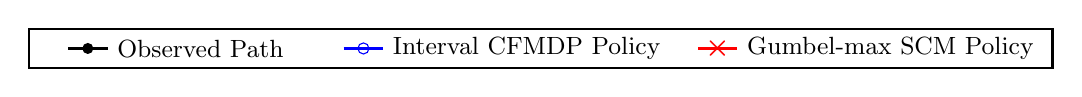
\begin{tikzpicture}[scale=1.0, every node/.style={scale=1.0}]
            \draw[thick, black] (-3, -0.25) rectangle (10, 0.25);
            %
            \draw[black, line width=1pt] (-2.5, 0.0) -- (-2,0.0);
            \fill[black] (-2.25,0.0) circle (2pt); %
            \node[right] at (-2,0.0) {\small Observed Path};
            
            %
            \draw[blue, line width=1pt] (1.0,0.0) -- (1.5,0.0);
            \node[draw=blue, circle, minimum size=4pt, inner sep=0pt] at (1.25,0.0) {}; %
            \node[right] at (1.5,0.0) {\small Interval CFMDP Policy};
            
            %
            \draw[red, line width=1pt] (5.5,0) -- (6,0);
            \node[red] at (5.75,0) {$\boldsymbol{\times}$}; %
            \node[right] at (6,0) {\small Gumbel-max SCM Policy};
        \end{tikzpicture}
    }\\
    %
    \subfigure[\footnotesize Lowest cumulative reward: Interval CFMDP ($312$), Gumbel-max SCM ($312$)]{%
        \resizebox{0.76\columnwidth}{!}{
             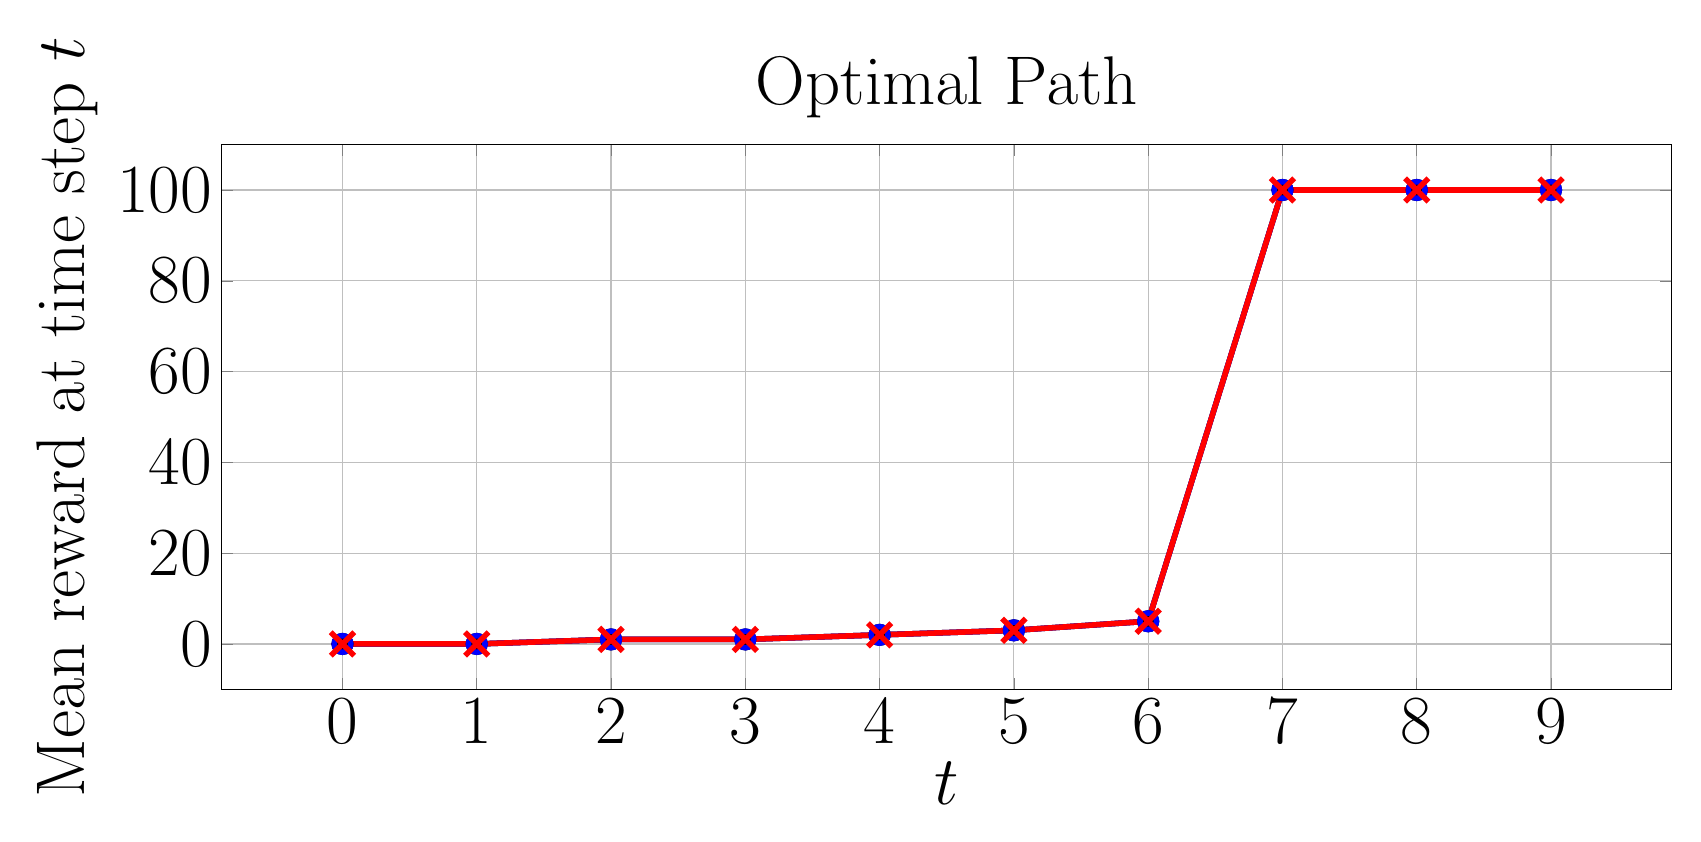
\begin{tikzpicture}
                \begin{axis}[
                    xlabel={$t$},
                    ylabel={Mean reward at time step $t$},
                    title={Optimal Path},
                    grid=both,
                    width=20cm, height=8.5cm,
                    every axis/.style={font=\Huge},
                    %
                ]
                \addplot[
                    color=black, %
                    mark=*, %
                    line width=2pt,
                    mark size=3pt,
                    error bars/.cd,
                    y dir=both, %
                    y explicit, %
                    error bar style={line width=1pt,solid},
                    error mark options={line width=1pt,mark size=4pt,rotate=90}
                ]
                coordinates {
                    (0, 0.0)  +- (0, 0.0)
                    (1, 0.0)  +- (0, 0.0) 
                    (2, 1.0)  +- (0, 0.0) 
                    (3, 1.0)  +- (0, 0.0)
                    (4, 2.0)  +- (0, 0.0)
                    (5, 3.0) +- (0, 0.0)
                    (6, 5.0) +- (0, 0.0)
                    (7, 100.0) +- (0, 0.0)
                    (8, 100.0) +- (0, 0.0)
                    (9, 100.0) +- (0, 0.0)
                };
                %
                \addplot[
                    color=blue, %
                    mark=o, %
                    line width=2pt,
                    mark size=3pt,
                    error bars/.cd,
                    y dir=both, %
                    y explicit, %
                    error bar style={line width=1pt,solid},
                    error mark options={line width=1pt,mark size=4pt,rotate=90}
                ]
                 coordinates {
                    (0, 0.0)  +- (0, 0.0)
                    (1, 0.0)  +- (0, 0.0) 
                    (2, 1.0)  +- (0, 0.0) 
                    (3, 1.0)  +- (0, 0.0)
                    (4, 2.0)  +- (0, 0.0)
                    (5, 3.0) +- (0, 0.0)
                    (6, 5.0) +- (0, 0.0)
                    (7, 100.0) +- (0, 0.0)
                    (8, 100.0) +- (0, 0.0)
                    (9, 100.0) +- (0, 0.0)
                };
                %
                \addplot[
                    color=red, %
                    mark=x, %
                    line width=2pt,
                    mark size=6pt,
                    error bars/.cd,
                    y dir=both, %
                    y explicit, %
                    error bar style={line width=1pt,solid},
                    error mark options={line width=1pt,mark size=4pt,rotate=90}
                ]
                coordinates {
                    (0, 0.0)  +- (0, 0.0)
                    (1, 0.0)  +- (0, 0.0) 
                    (2, 1.0)  +- (0, 0.0) 
                    (3, 1.0)  +- (0, 0.0)
                    (4, 2.0)  +- (0, 0.0)
                    (5, 3.0) +- (0, 0.0)
                    (6, 5.0) +- (0, 0.0)
                    (7, 100.0) +- (0, 0.0)
                    (8, 100.0) +- (0, 0.0)
                    (9, 100.0) +- (0, 0.0)
                };
                \end{axis}
            \end{tikzpicture}
         }
    }
    \hspace{1cm}
    \subfigure[\footnotesize Lowest cumulative reward: Interval CFMDP ($19$), Gumbel-max SCM ($-88$)]{%
         \resizebox{0.76\columnwidth}{!}{
            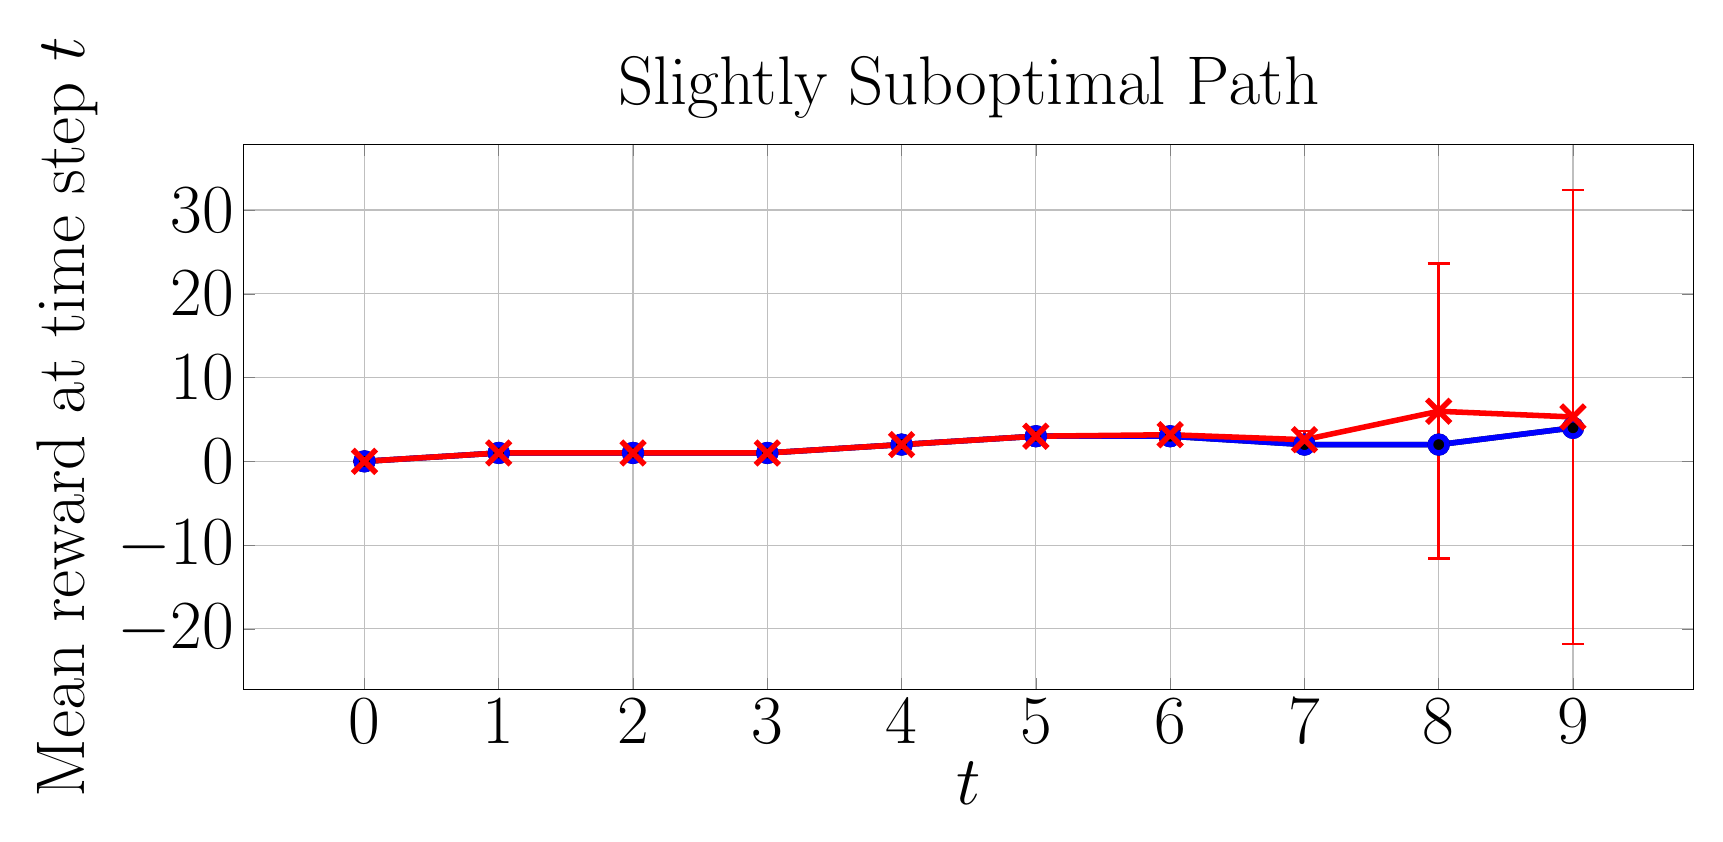
\begin{tikzpicture}
                \begin{axis}[
                    xlabel={$t$},
                    ylabel={Mean reward at time step $t$},
                    title={Slightly Suboptimal Path},
                    grid=both,
                    width=20cm, height=8.5cm,
                    every axis/.style={font=\Huge},
                    %
                ]
                \addplot[
                    color=black, %
                    mark=*, %
                    line width=2pt,
                    mark size=3pt,
                    error bars/.cd,
                    y dir=both, %
                    y explicit, %
                    error bar style={line width=1pt,solid},
                    error mark options={line width=1pt,mark size=4pt,rotate=90}
                ]
              coordinates {
                    (0, 0.0)  +- (0, 0.0)
                    (1, 1.0)  +- (0, 0.0) 
                    (2, 1.0)  +- (0, 0.0) 
                    (3, 1.0)  +- (0, 0.0)
                    (4, 2.0)  +- (0, 0.0)
                    (5, 3.0) +- (0, 0.0)
                    (6, 3.0) +- (0, 0.0)
                    (7, 2.0) +- (0, 0.0)
                    (8, 2.0) +- (0, 0.0)
                    (9, 4.0) +- (0, 0.0)
                };
                %
                \addplot[
                    color=blue, %
                    mark=o, %
                    line width=2pt,
                    mark size=3pt,
                    error bars/.cd,
                    y dir=both, %
                    y explicit, %
                    error bar style={line width=1pt,solid},
                    error mark options={line width=1pt,mark size=4pt,rotate=90}
                ]
              coordinates {
                    (0, 0.0)  +- (0, 0.0)
                    (1, 1.0)  +- (0, 0.0) 
                    (2, 1.0)  +- (0, 0.0) 
                    (3, 1.0)  +- (0, 0.0)
                    (4, 2.0)  +- (0, 0.0)
                    (5, 3.0) +- (0, 0.0)
                    (6, 3.0) +- (0, 0.0)
                    (7, 2.0) +- (0, 0.0)
                    (8, 2.0) +- (0, 0.0)
                    (9, 4.0) +- (0, 0.0)
                };
                %
                \addplot[
                    color=red, %
                    mark=x, %
                    line width=2pt,
                    mark size=6pt,
                    error bars/.cd,
                    y dir=both, %
                    y explicit, %
                    error bar style={line width=1pt,solid},
                    error mark options={line width=1pt,mark size=4pt,rotate=90}
                ]
                coordinates {
                    (0, 0.0)  +- (0, 0.0)
                    (1, 1.0)  +- (0, 0.0) 
                    (2, 1.0)  +- (0, 0.0) 
                    (3, 1.0)  +- (0, 0.0)
                    (4, 2.0)  += (0, 0.0)
                    (5, 3.0)  += (0, 0.0)
                    (6, 3.17847) += (0, 0.62606746) -= (0, 0.62606746)
                    (7, 2.5832885) += (0, 1.04598233) -= (0, 1.04598233)
                    (8, 5.978909) += (0, 17.60137623) -= (0, 17.60137623)
                    (9, 5.297059) += (0, 27.09227512) -= (0, 27.09227512)
                };
                \end{axis}
            \end{tikzpicture}
         }
    }\\[-1.5pt]
    \subfigure[\footnotesize Lowest cumulative reward: Interval CFMDP ($14$), Gumbel-max SCM ($-598$)]{%
         \resizebox{0.76\columnwidth}{!}{
             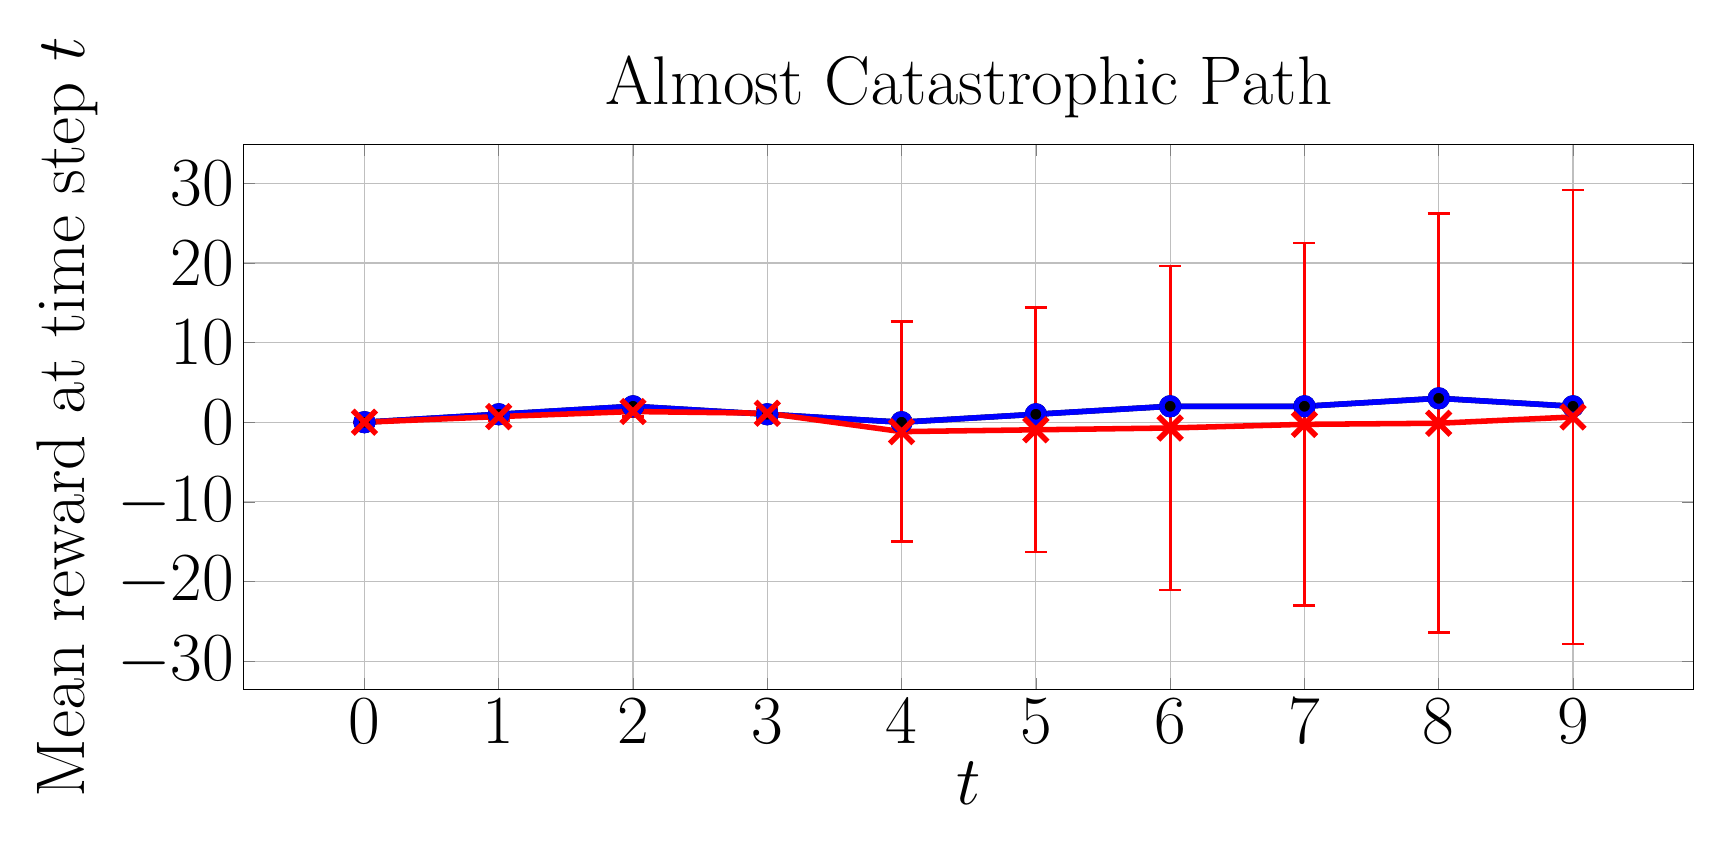
\begin{tikzpicture}
                \begin{axis}[
                    xlabel={$t$},
                    ylabel={Mean reward at time step $t$},
                    title={Almost Catastrophic Path},
                    grid=both,
                    width=20cm, height=8.5cm,
                    every axis/.style={font=\Huge},
                    %
                ]
                \addplot[
                    color=black, %
                    mark=*, %
                    line width=2pt,
                    mark size=3pt,
                    error bars/.cd,
                    y dir=both, %
                    y explicit, %
                    error bar style={line width=1pt,solid},
                    error mark options={line width=1pt,mark size=4pt,rotate=90}
                ]
                coordinates {
                    (0, 0.0)  +- (0, 0.0)
                    (1, 1.0)  +- (0, 0.0) 
                    (2, 2.0)  +- (0, 0.0) 
                    (3, 1.0)  +- (0, 0.0)
                    (4, 0.0)  +- (0, 0.0)
                    (5, 1.0) +- (0, 0.0)
                    (6, 2.0) +- (0, 0.0)
                    (7, 2.0) +- (0, 0.0)
                    (8, 3.0) +- (0, 0.0)
                    (9, 2.0) +- (0, 0.0)
                };
                %
                \addplot[
                    color=blue, %
                    mark=o, %
                    line width=2pt,
                    mark size=3pt,
                    error bars/.cd,
                    y dir=both, %
                    y explicit, %
                    error bar style={line width=1pt,solid},
                    error mark options={line width=1pt,mark size=4pt,rotate=90}
                ]
                coordinates {
                    (0, 0.0)  +- (0, 0.0)
                    (1, 1.0)  +- (0, 0.0) 
                    (2, 2.0)  +- (0, 0.0) 
                    (3, 1.0)  +- (0, 0.0)
                    (4, 0.0)  +- (0, 0.0)
                    (5, 1.0) +- (0, 0.0)
                    (6, 2.0) +- (0, 0.0)
                    (7, 2.0) +- (0, 0.0)
                    (8, 3.0) +- (0, 0.0)
                    (9, 2.0) +- (0, 0.0)
                };
                %
                \addplot[
                    color=red, %
                    mark=x, %
                    line width=2pt,
                    mark size=6pt,
                    error bars/.cd,
                    y dir=both, %
                    y explicit, %
                    error bar style={line width=1pt,solid},
                    error mark options={line width=1pt,mark size=4pt,rotate=90}
                ]
                coordinates {
                    (0, 0.0)  +- (0, 0.0)
                    (1, 0.7065655)  +- (0, 0.4553358) 
                    (2, 1.341673)  +- (0, 0.67091621) 
                    (3, 1.122926)  +- (0, 0.61281824)
                    (4, -1.1821935)  +- (0, 13.82444042)
                    (5, -0.952399)  +- (0, 15.35195457)
                    (6, -0.72672) +- (0, 20.33508414)
                    (7, -0.268983) +- (0, 22.77861454)
                    (8, -0.1310835) +- (0, 26.31013314)
                    (9, 0.65806) +- (0, 28.50670214)
                };
                %
            %
            %
            %
            %
            %
            %
            %
            %
            %
            %
            %
            %
            %
            %
            %
            %
            %
            %
                \end{axis}
            \end{tikzpicture}
         }
    }
    \hspace{1cm}
    \subfigure[\footnotesize Lowest cumulative reward: Interval CFMDP ($-698$), Gumbel-max SCM ($-698$)]{%
         \resizebox{0.76\columnwidth}{!}{
            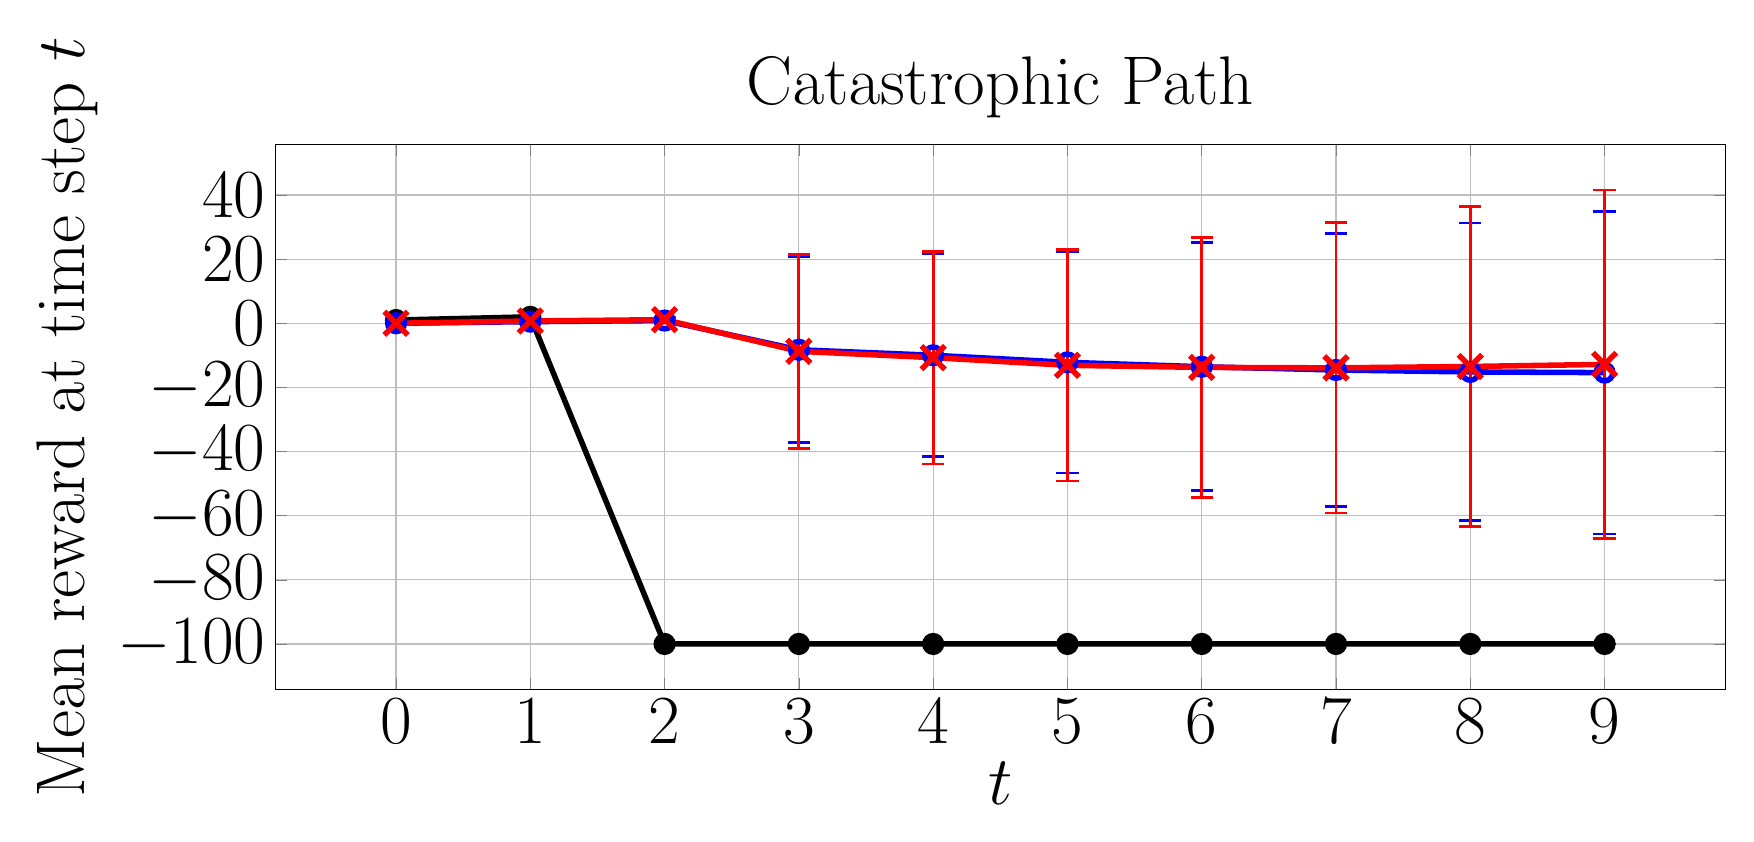
\begin{tikzpicture}
                \begin{axis}[
                    xlabel={$t$},
                    ylabel={Mean reward at time step $t$},
                    title={Catastrophic Path},
                    grid=both,
                    width=20cm, height=8.5cm,
                    every axis/.style={font=\Huge},
                    %
                ]
                \addplot[
                    color=black, %
                    mark=*, %
                    line width=2pt,
                    mark size=3pt,
                    error bars/.cd,
                    y dir=both, %
                    y explicit, %
                    error bar style={line width=1pt,solid},
                    error mark options={line width=1pt,mark size=4pt,rotate=90}
                ]
                coordinates {
                    (0, 1.0)  +- (0, 0.0)
                    (1, 2.0)  +- (0, 0.0) 
                    (2, -100.0)  +- (0, 0.0) 
                    (3, -100.0)  +- (0, 0.0)
                    (4, -100.0)  +- (0, 0.0)
                    (5, -100.0) +- (0, 0.0)
                    (6, -100.0) +- (0, 0.0)
                    (7, -100.0) +- (0, 0.0)
                    (8, -100.0) +- (0, 0.0)
                    (9, -100.0) +- (0, 0.0)
                };
                %
                \addplot[
                    color=blue, %
                    mark=o, %
                    line width=2pt,
                    mark size=3pt,
                    error bars/.cd,
                    y dir=both, %
                    y explicit, %
                    error bar style={line width=1pt,solid},
                    error mark options={line width=1pt,mark size=4pt,rotate=90}
                ]
                coordinates {
                    (0, 0.0)  +- (0, 0.0)
                    (1, 0.504814)  +- (0, 0.49997682) 
                    (2, 0.8439835)  +- (0, 0.76831917) 
                    (3, -8.2709165)  +- (0, 28.93656754)
                    (4, -9.981082)  +- (0, 31.66825363)
                    (5, -12.1776325) +- (0, 34.53463233)
                    (6, -13.556076) +- (0, 38.62845372)
                    (7, -14.574418) +- (0, 42.49603359)
                    (8, -15.1757075) +- (0, 46.41913968)
                    (9, -15.3900395) +- (0, 50.33563368)
                };
                %
                \addplot[
                    color=red, %
                    mark=x, %
                    line width=2pt,
                    mark size=6pt,
                    error bars/.cd,
                    y dir=both, %
                    y explicit, %
                    error bar style={line width=1pt,solid},
                    error mark options={line width=1pt,mark size=4pt,rotate=90}
                ]
                coordinates {
                    (0, 0.0)  +- (0, 0.0)
                    (1, 0.701873)  +- (0, 0.45743556) 
                    (2, 1.1227805)  +- (0, 0.73433129) 
                    (3, -8.7503255)  +- (0, 30.30257976)
                    (4, -10.722092)  +- (0, 33.17618589)
                    (5, -13.10721)  +- (0, 36.0648089)
                    (6, -13.7631645) +- (0, 40.56553451)
                    (7, -13.909043) +- (0, 45.23829402)
                    (8, -13.472517) +- (0, 49.96270296)
                    (9, -12.8278835) +- (0, 54.38618735)
                };
                %
            %
            %
            %
            %
            %
            %
            %
            %
            %
            %
            %
            %
            %
            %
            %
            %
            %
            %
                \end{axis}
            \end{tikzpicture}
         }
    }
    \caption{Average instant reward of CF paths induced by policies on GridWorld $p=0.4$.}
    \label{fig: reward p=0.4}
\end{figure*}

\subsection{Experimental Setup}
To compare policy performance, we measure the average rewards of counterfactual paths induced by our policy and the Gumbel-max policy by uniformly sampling $200$ counterfactual MDPs from the ICFMDP and generating $10,000$ counterfactual paths over each sampled CFMDP. \jl{Since the interval CFMDP depends on the observed path, we select $4$  paths of varying optimality to evaluate how the observed path impacts the performance of both policies: an optimal path, a slightly suboptimal path that could reach the optimal reward with a few changes, a catastrophic path that enters a catastrophic, terminal state with low reward, and an almost catastrophic path that was close to entering a catastrophic state.} When measuring the average probability bound widths and execution time needed to generate the ICFMDPs, we averaged over $20$ randomly generated observed paths
\footnote{Further training details are provided in Appendix \ref{app: training details}, and the code is provided at \href{https://github.com/ddv-lab/robust-cf-inference-in-MDPs}{https://github.com/ddv-lab/robust-cf-inference-in-MDPs}
%
%
.}.

\subsection{GridWorld}
\jl{The GridWorld MDP is a $4 \times 4$ grid where an agent must navigate from the top-left corner to the goal state in the bottom-right corner, avoiding a dangerous terminal state in the centre. At each time step, the agent can move up, down, left, or right, but there is a small probability (controlled by hyper-parameter $p$) of moving in an unintended direction. As the agent nears the goal, the reward for each state increases, culminating in a reward of $+100$ for reaching the goal. Entering the dangerous state results in a penalty of $-100$. We use two versions of GridWorld: a less stochastic version with $p=0.9$ (i.e., $90$\% chance of moving in the chosen direction) and a more stochastic version with $p=0.4$.}

\paragraph{GridWorld ($p=0.9$)}
When $p=0.9$, the counterfactual probability bounds are typically narrow (see Table \ref{tab:nonzero_probs} for average measurements). Consequently, as shown in Figure \ref{fig: reward p=0.9}, both policies are nearly identical and perform similarly well across the optimal, slightly suboptimal, and catastrophic paths.
%
However, for the almost catastrophic path, the interval CFMDP path is more conservative and follows the observed path more closely (as this is where the probability bounds are narrowest), which typically requires one additional step to reach the goal state than the Gumbel-max SCM policy.
%

\paragraph{GridWorld ($p=0.4$)}
\jl{When $p=0.4$, the GridWorld environment becomes more uncertain, increasing the risk of entering the dangerous state even if correct actions are chosen. Thus, as shown in Figure \ref{fig: reward p=0.4}, the interval CFMDP policy adopts a more conservative approach, avoiding deviation from the observed policy if it cannot guarantee higher counterfactual rewards (see the slightly suboptimal and almost catastrophic paths), whereas the Gumbel-max SCM is inconsistent: it can yield higher rewards, but also much lower rewards, reflected in the wide error bars.} For the catastrophic path, both policies must deviate from the observed path to achieve a higher reward and, in this case, perform similarly.
%
%
%
%
\subsection{Sepsis}
The Sepsis MDP \citep{oberst2019counterfactual} simulates trajectories of Sepsis patients. Each state consists of four vital signs (heart rate, blood pressure, oxygen concentration, and glucose levels), categorised as low, normal, or high.
and three treatments that can be toggled on/off at each time step (8 actions in total). Unlike \citet{oberst2019counterfactual}, we scale rewards based on the number of out-of-range vital signs, between $-1000$ (patient dies) and $1000$ (patient discharged). \jl{Like the GridWorld $p=0.4$ experiment, the Sepsis MDP is highly uncertain, as many states are equally likely to lead to optimal and poor outcomes. Thus, as shown in Figure \ref{fig: reward sepsis}, both policies follow the observed optimal and almost catastrophic paths to guarantee rewards are no worse than the observation.} However, improving the catastrophic path requires deviating from the observation. Here, the Gumbel-max SCM policy, on average, performs better than the interval CFMDP policy. But, since both policies have lower bounds clipped at $-1000$, neither policy reliably improves over the observation. In contrast, for the slightly suboptimal path, the interval CFMDP policy performs significantly better, shown by its higher lower bounds. 
Moreover, in these two cases, the worst-case counterfactual path generated by the interval CFMDP policy is better than that of the Gumbel-max SCM policy,
indicating its greater robustness.
%
\begin{figure*}
    \centering
     \resizebox{0.6\textwidth}{!}{
        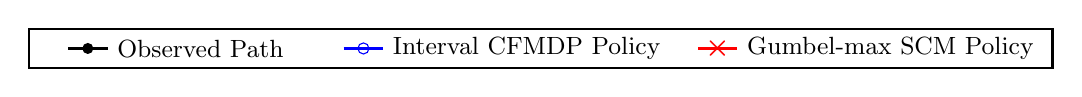
\begin{tikzpicture}[scale=1.0, every node/.style={scale=1.0}]
            \draw[thick, black] (-3, -0.25) rectangle (10, 0.25);
            %
            \draw[black, line width=1pt] (-2.5, 0.0) -- (-2,0.0);
            \fill[black] (-2.25,0.0) circle (2pt); %
            \node[right] at (-2,0.0) {\small Observed Path};
            
            %
            \draw[blue, line width=1pt] (1.0,0.0) -- (1.5,0.0);
            \node[draw=blue, circle, minimum size=4pt, inner sep=0pt] at (1.25,0.0) {}; %
            \node[right] at (1.5,0.0) {\small Interval CFMDP Policy};
            
            %
            \draw[red, line width=1pt] (5.5,0) -- (6,0);
            \node[red] at (5.75,0) {$\boldsymbol{\times}$}; %
            \node[right] at (6,0) {\small Gumbel-max SCM Policy};
        \end{tikzpicture}
    }\\
    \subfigure[\footnotesize Lowest cumulative reward: Interval CFMDP ($8000$), Gumbel-max SCM ($8000$)]{%
         \resizebox{0.76\columnwidth}{!}{
             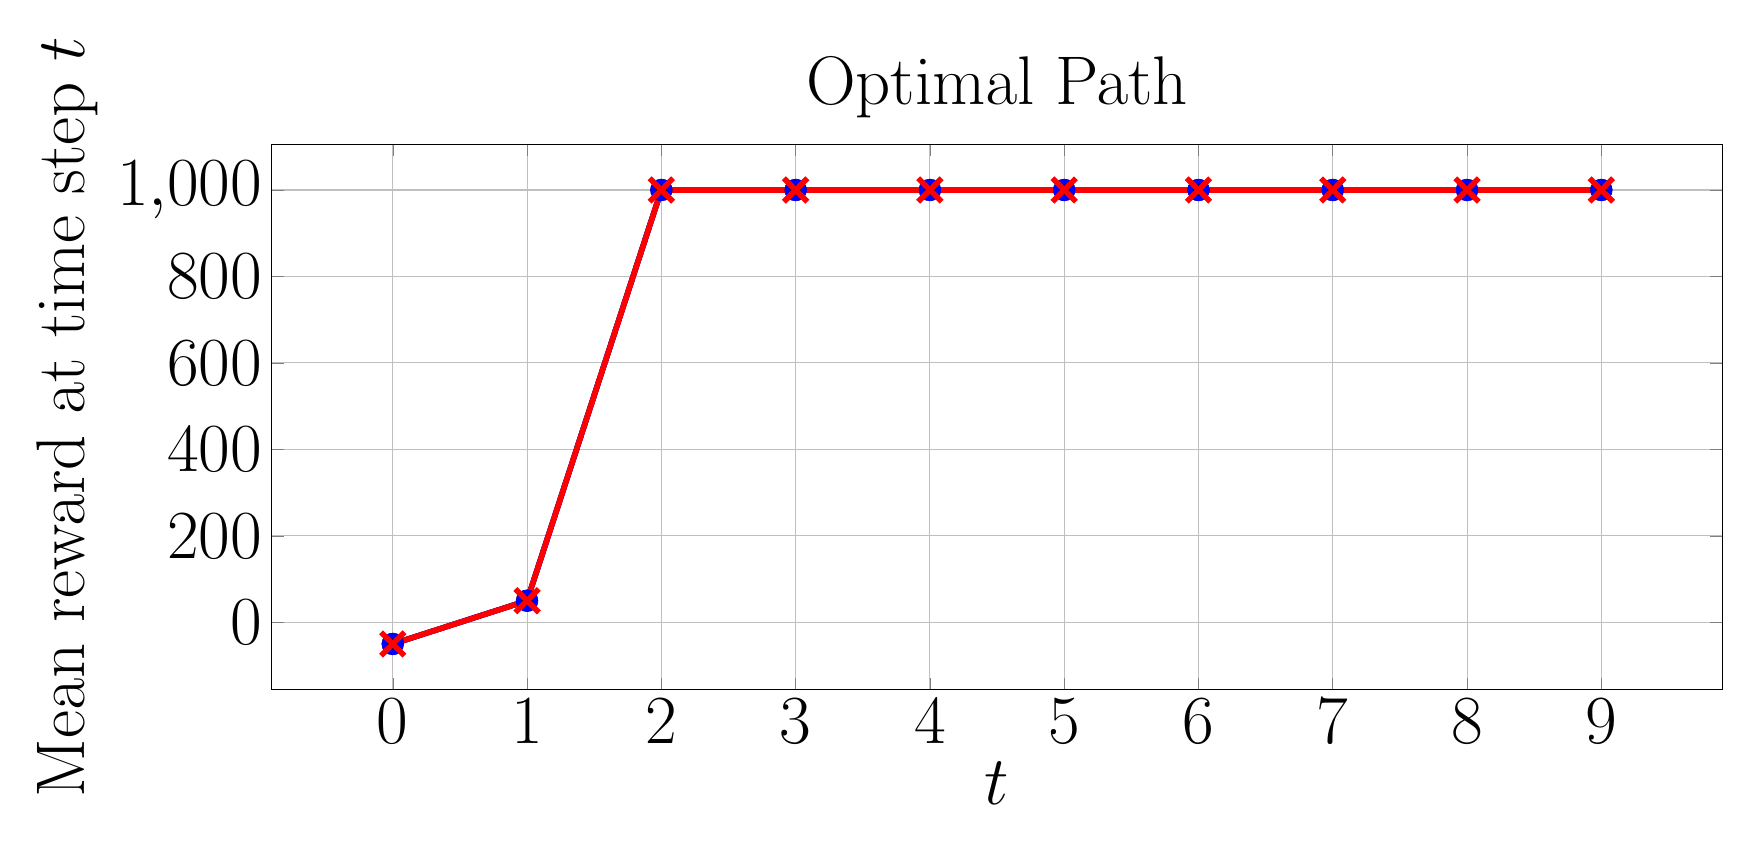
\begin{tikzpicture}
                \begin{axis}[
                    xlabel={$t$},
                    ylabel={Mean reward at time step $t$},
                    title={Optimal Path},
                    grid=both,
                    width=20cm, height=8.5cm,
                    every axis/.style={font=\Huge},
                    %
                ]
                \addplot[
                    color=black, %
                    mark=*, %
                    line width=2pt,
                    mark size=3pt,
                ]
                coordinates {
                    (0, -50.0)
                    (1, 50.0)
                    (2, 1000.0)
                    (3, 1000.0)
                    (4, 1000.0)
                    (5, 1000.0)
                    (6, 1000.0)
                    (7, 1000.0)
                    (8, 1000.0)
                    (9, 1000.0)
                };
                %
                \addplot[
                    color=blue, %
                    mark=o, %
                    line width=2pt,
                    mark size=3pt,
                    error bars/.cd,
                    y dir=both, %
                    y explicit, %
                    error bar style={line width=1pt,solid},
                    error mark options={line width=1pt,mark size=4pt,rotate=90}
                ]
                coordinates {
                    (0, -50.0)  +- (0, 0.0)
                    (1, 50.0)  +- (0, 0.0) 
                    (2, 1000.0)  +- (0, 0.0) 
                    (3, 1000.0)  +- (0, 0.0)
                    (4, 1000.0)  +- (0, 0.0)
                    (5, 1000.0) +- (0, 0.0)
                    (6, 1000.0) +- (0, 0.0)
                    (7, 1000.0) +- (0, 0.0)
                    (8, 1000.0) +- (0, 0.0)
                    (9, 1000.0) +- (0, 0.0)
                };
                %
                \addplot[
                    color=red, %
                    mark=x, %
                    line width=2pt,
                    mark size=6pt,
                    error bars/.cd,
                    y dir=both, %
                    y explicit, %
                    error bar style={line width=1pt,solid},
                    error mark options={line width=1pt,mark size=4pt,rotate=90}
                ]
                coordinates {
                    (0, -50.0)  +- (0, 0.0)
                    (1, 50.0)  +- (0, 0.0) 
                    (2, 1000.0)  +- (0, 0.0) 
                    (3, 1000.0)  +- (0, 0.0)
                    (4, 1000.0)  +- (0, 0.0)
                    (5, 1000.0) +- (0, 0.0)
                    (6, 1000.0) +- (0, 0.0)
                    (7, 1000.0) +- (0, 0.0)
                    (8, 1000.0) +- (0, 0.0)
                    (9, 1000.0) +- (0, 0.0)
                };
                %
                \end{axis}
            \end{tikzpicture}
         }
    }
    \hspace{1cm}
    \subfigure[\footnotesize Lowest cumulative reward: Interval CFMDP ($-5980$), Gumbel-max SCM ($-8000$)]{%
         \resizebox{0.76\columnwidth}{!}{
            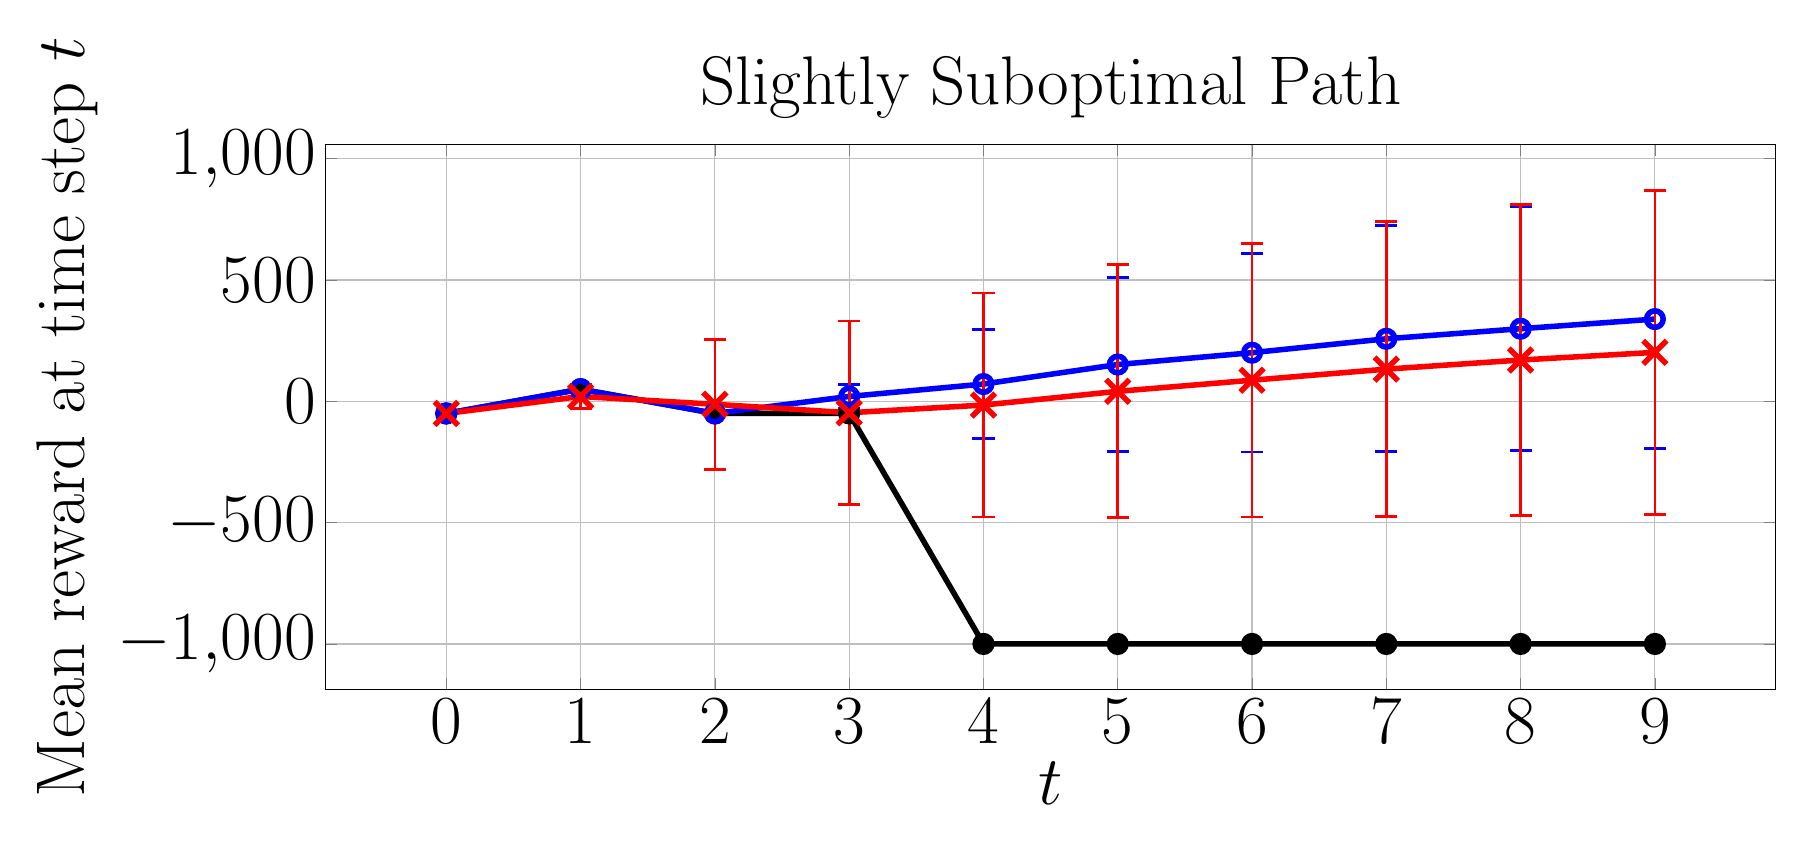
\begin{tikzpicture}
                \begin{axis}[
                    xlabel={$t$},
                    ylabel={Mean reward at time step $t$},
                    title={Slightly Suboptimal Path},
                    grid=both,
                    width=20cm, height=8.5cm,
                    every axis/.style={font=\Huge},
                    %
                ]
               \addplot[
                    color=black, %
                    mark=*, %
                    line width=2pt,
                    mark size=3pt,
                ]
                coordinates {
                    (0, -50.0)
                    (1, 50.0)
                    (2, -50.0)
                    (3, -50.0)
                    (4, -1000.0)
                    (5, -1000.0)
                    (6, -1000.0)
                    (7, -1000.0)
                    (8, -1000.0)
                    (9, -1000.0)
                };
                %
                \addplot[
                    color=blue, %
                    mark=o, %
                    line width=2pt,
                    mark size=3pt,
                    error bars/.cd,
                    y dir=both, %
                    y explicit, %
                    error bar style={line width=1pt,solid},
                    error mark options={line width=1pt,mark size=4pt,rotate=90}
                ]
                coordinates {
                    (0, -50.0)  +- (0, 0.0)
                    (1, 50.0)  +- (0, 0.0) 
                    (2, -50.0)  +- (0, 0.0) 
                    (3, 20.0631)  +- (0, 49.97539413)
                    (4, 71.206585)  +- (0, 226.02033693)
                    (5, 151.60797) +- (0, 359.23292559)
                    (6, 200.40593) +- (0, 408.86185176)
                    (7, 257.77948) +- (0, 466.10372804)
                    (8, 299.237465) +- (0, 501.82579506)
                    (9, 338.9129) +- (0, 532.06124996)
                };
                %
                \addplot[
                    color=red, %
                    mark=x, %
                    line width=2pt,
                    mark size=6pt,
                    error bars/.cd,
                    y dir=both, %
                    y explicit, %
                    error bar style={line width=1pt,solid},
                    error mark options={line width=1pt,mark size=4pt,rotate=90}
                ]
                coordinates {
                    (0, -50.0)  +- (0, 0.0)
                    (1, 20.00736)  +- (0, 49.99786741) 
                    (2, -12.282865)  +- (0, 267.598755) 
                    (3, -47.125995)  +- (0, 378.41755832)
                    (4, -15.381965)  +- (0, 461.77616558)
                    (5, 41.15459) +- (0, 521.53189262)
                    (6, 87.01595) +- (0, 564.22243126 )
                    (7, 132.62376) +- (0, 607.31338037)
                    (8, 170.168145) +- (0, 641.48013693)
                    (9, 201.813135) +- (0, 667.29441777)
                };
                %
                %
                %
                %
                %
                %
                %
                %
                %
                %
                %
                %
                %
                %
                %
                %
                %
                %
                %
                \end{axis}
            \end{tikzpicture}
         }
    }\\[-1.5pt]
    \subfigure[\footnotesize Lowest cumulative reward: Interval CFMDP ($100$), Gumbel-max SCM ($100$)]{%
         \resizebox{0.76\columnwidth}{!}{
             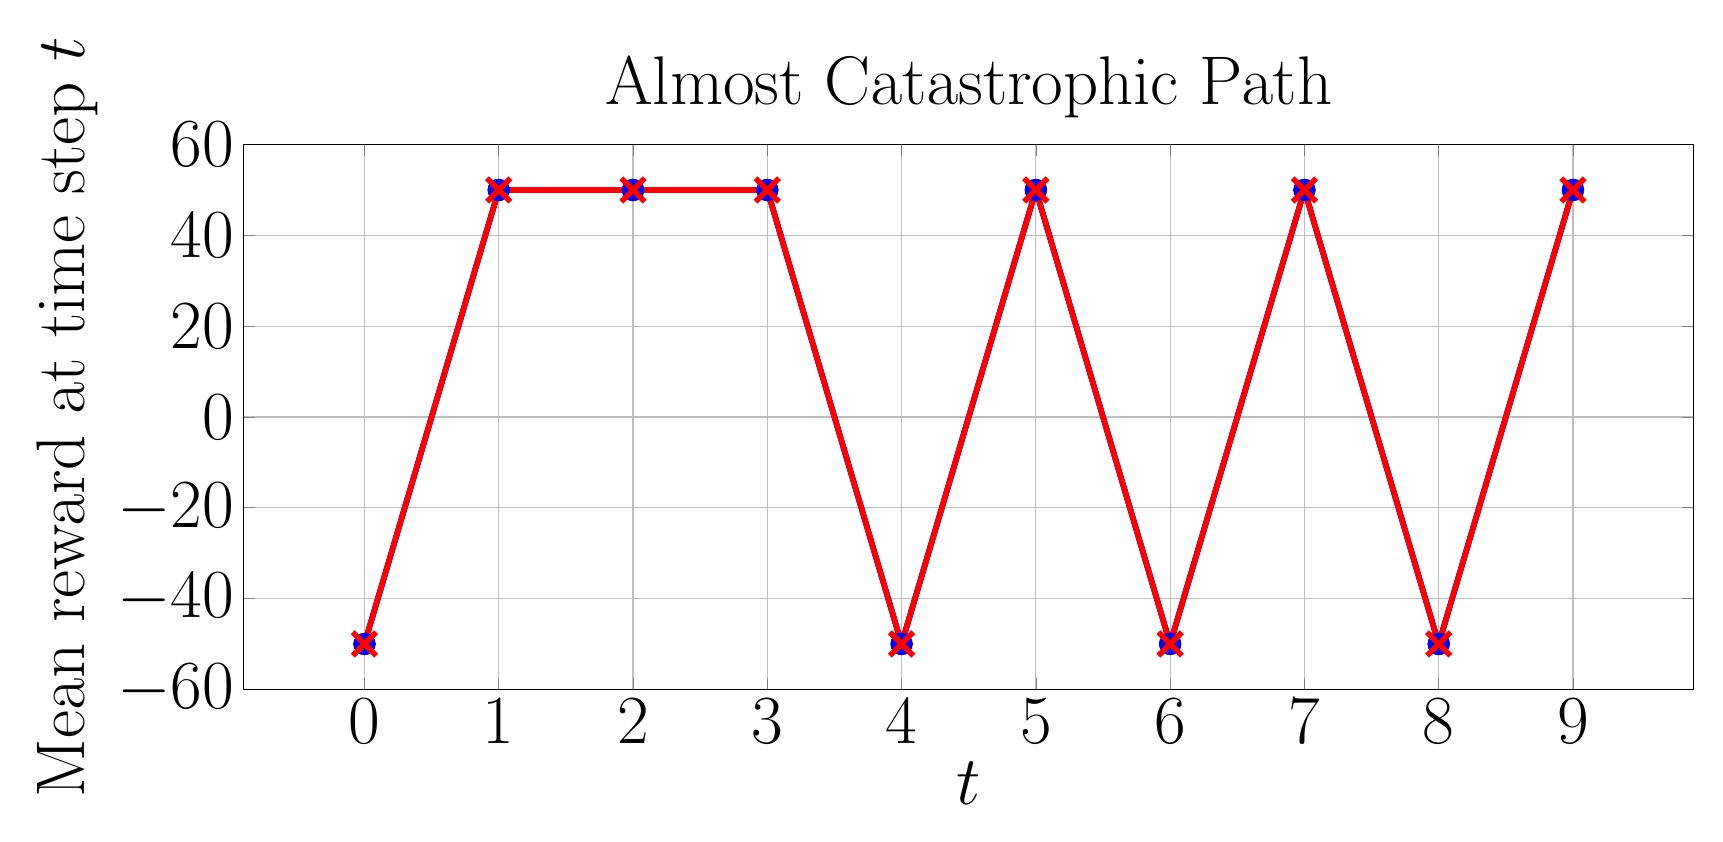
\begin{tikzpicture}
                \begin{axis}[
                    xlabel={$t$},
                    ylabel={Mean reward at time step $t$},
                    title={Almost Catastrophic Path},
                    grid=both,
                    every axis/.style={font=\Huge},
                    width=20cm, height=8.5cm,
                    %
                ]
               \addplot[
                    color=black, %
                    mark=*, %
                    line width=2pt,
                    mark size=3pt,
                ]
                coordinates {
                    (0, -50.0)
                    (1, 50.0)
                    (2, 50.0)
                    (3, 50.0)
                    (4, -50.0)
                    (5, 50.0)
                    (6, -50.0)
                    (7, 50.0)
                    (8, -50.0)
                    (9, 50.0)
                };
                %
                %
                \addplot[
                    color=blue, %
                    mark=o, %
                    line width=2pt,
                    mark size=3pt,
                    error bars/.cd,
                    y dir=both, %
                    y explicit, %
                    error bar style={line width=1pt,solid},
                    error mark options={line width=1pt,mark size=4pt,rotate=90}
                ]
                coordinates {
                    (0, -50.0)  +- (0, 0.0)
                    (1, 50.0)  +- (0, 0.0) 
                    (2, 50.0)  +- (0, 0.0) 
                    (3, 50.0)  +- (0, 0.0)
                    (4, -50.0)  +- (0, 0.0)
                    (5, 50.0) +- (0, 0.0)
                    (6, -50.0) +- (0, 0.0)
                    (7, 50.0) +- (0, 0.0)
                    (8, -50.0) +- (0, 0.0)
                    (9, 50.0) +- (0, 0.0)
                };
                %
                \addplot[
                    color=red, %
                    mark=x, %
                    line width=2pt,
                    mark size=6pt,
                    error bars/.cd,
                    y dir=both, %
                    y explicit, %
                    error bar style={line width=1pt,solid},
                    error mark options={line width=1pt,mark size=4pt,rotate=90}
                ]
                coordinates {
                    (0, -50.0)  +- (0, 0.0)
                    (1, 50.0)  +- (0, 0.0) 
                    (2, 50.0)  +- (0, 0.0) 
                    (3, 50.0)  +- (0, 0.0)
                    (4, -50.0)  +- (0, 0.0)
                    (5, 50.0) +- (0, 0.0)
                    (6, -50.0) +- (0, 0.0)
                    (7, 50.0) +- (0, 0.0)
                    (8, -50.0) +- (0, 0.0)
                    (9, 50.0) +- (0, 0.0)
                };
                %
                %
                %
                %
                %
                %
                %
                %
                %
                %
                %
                %
                %
                %
                %
                %
                %
                %
                %
                \end{axis}
            \end{tikzpicture}
         }
    }
    \hspace{1cm}
    \subfigure[\footnotesize Lowest cumulative reward: Interval CFMDP ($-7150$), Gumbel-max SCM ($-9050$)]{%
         \resizebox{0.76\columnwidth}{!}{
            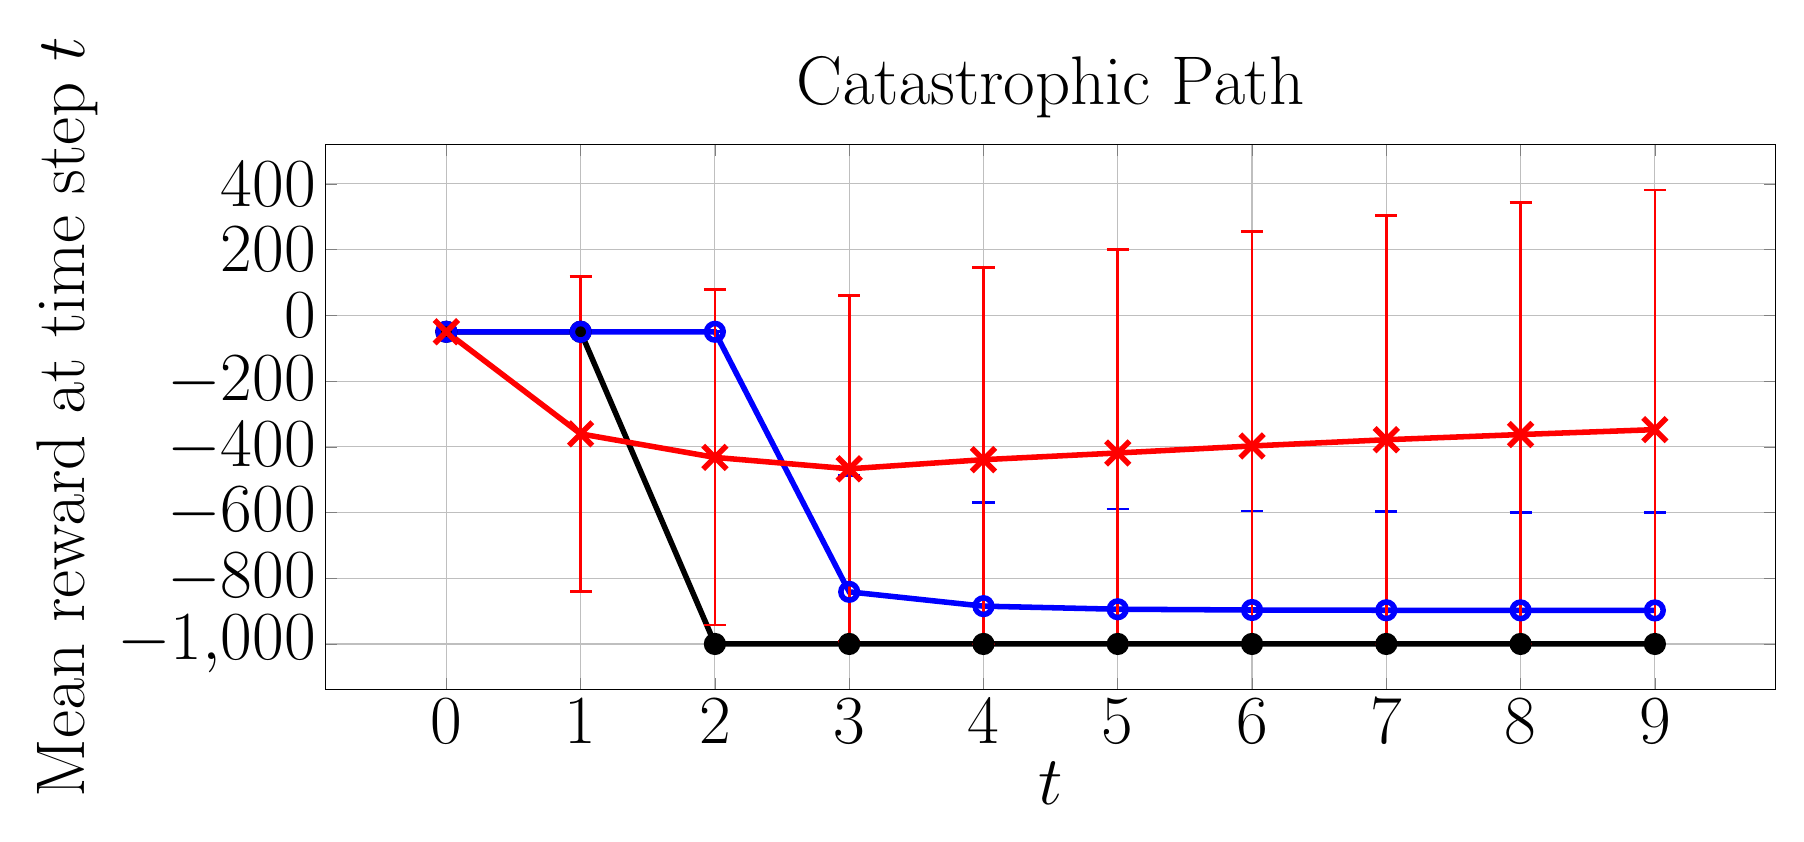
\begin{tikzpicture}
                \begin{axis}[
                    xlabel={$t$},
                    ylabel={Mean reward at time step $t$},
                    title={Catastrophic Path},
                    grid=both,
                    width=20cm, height=8.5cm,
                    every axis/.style={font=\Huge},
                    %
                ]
               \addplot[
                    color=black, %
                    mark=*, %
                    line width=2pt,
                    mark size=3pt,
                ]
                coordinates {
                    (0, -50.0)
                    (1, -50.0)
                    (2, -1000.0)
                    (3, -1000.0)
                    (4, -1000.0)
                    (5, -1000.0)
                    (6, -1000.0)
                    (7, -1000.0)
                    (8, -1000.0)
                    (9, -1000.0)
                };
                %
                %
                \addplot[
                    color=blue, %
                    mark=o, %
                    line width=2pt,
                    mark size=3pt,
                    error bars/.cd,
                    y dir=both, %
                    y explicit, %
                    error bar style={line width=1pt,solid},
                    error mark options={line width=1pt,mark size=4pt,rotate=90}
                ]
                coordinates {
                    (0, -50.0)  +- (0, 0.0)
                    (1, -50.0)  +- (0, 0.0) 
                    (2, -50.0)  +- (0, 0.0) 
                    (3, -841.440725)  += (0, 354.24605512) -= (0, 158.559275)
                    (4, -884.98225)  += (0, 315.37519669) -= (0, 115.01775)
                    (5, -894.330425) += (0, 304.88572805) -= (0, 105.669575)
                    (6, -896.696175) += (0, 301.19954514) -= (0, 103.303825)
                    (7, -897.4635) += (0, 299.61791279) -= (0, 102.5365)
                    (8, -897.77595) += (0, 298.80392585) -= (0, 102.22405)
                    (9, -897.942975) += (0, 298.32920557) -= (0, 102.057025)
                };
                %
                \addplot[
                    color=red, %
                    mark=x, %
                    line width=2pt,
                    mark size=6pt,
                    error bars/.cd,
                    y dir=both, %
                    y explicit, %
                    error bar style={line width=1pt,solid},
                    error mark options={line width=1pt,mark size=4pt,rotate=90}
                ]
            coordinates {
                    (0, -50.0)  +- (0, 0.0)
                    (1, -360.675265)  +- (0, 479.39812699) 
                    (2, -432.27629)  +- (0, 510.38620897) 
                    (3, -467.029545)  += (0, 526.36009628) -= (0, 526.36009628)
                    (4, -439.17429)  += (0, 583.96638919) -= (0, 560.82571)
                    (5, -418.82704) += (0, 618.43027478) -= (0, 581.17296)
                    (6, -397.464895) += (0, 652.67322574) -= (0, 602.535105)
                    (7, -378.49052) += (0, 682.85407033) -= (0, 621.50948)
                    (8, -362.654195) += (0, 707.01412023) -= (0, 637.345805)
                    (9, -347.737935) += (0, 729.29076479) -= (0, 652.262065)
                };
                %
                %
                %
                %
                %
                %
                %
                %
                %
                %
                %
                %
                %
                %
                %
                %
                %
                %
                %
                \end{axis}
            \end{tikzpicture}
         }
    }
    \caption{Average instant reward of CF paths induced by policies on Sepsis.}
    \label{fig: reward sepsis}
\end{figure*}

%
%
%
\subsection{Interval CFMDP Bounds}
%
%
Table \ref{tab:nonzero_probs} presents the mean counterfactual probability bound widths (excluding transitions where the upper bound is $0$) for each MDP, averaged over 20 observed paths. We compare the bounds under counterfactual stability (CS) and monotonicity (M) assumptions, CS alone, and no assumptions. This shows that the assumptions marginally reduce the bound widths, indicating the assumptions tighten the bounds without excluding too many causal models, as intended.
\renewcommand{\arraystretch}{1}

\begin{table}
\centering
\caption{Mean width of counterfactual probability bounds}
\resizebox{0.8\columnwidth}{!}{%
\begin{tabular}{|c|c|c|c|}
\hline
\multirow{2}{*}{\textbf{Environment}} & \multicolumn{3}{c|}{\textbf{Assumptions}} \\ \cline{2-4}
 & \textbf{CS + M} & \textbf{CS} & \textbf{None\tablefootnote{\jl{Equivalent to \citet{li2024probabilities}'s bounds (see Section \ref{sec: equivalence with Li}).}}} \\ \hline
\textbf{GridWorld} ($p=0.9$) & 0.0817 & 0.0977 & 0.100 \\ \hline
\textbf{GridWorld} ($p=0.4$) & 0.552  & 0.638  & 0.646 \\ \hline
\textbf{Sepsis} & 0.138 & 0.140 & 0.140 \\ \hline
\end{tabular}
}
\label{tab:nonzero_probs}
\end{table}


\subsection{Execution Times}
Table \ref{tab: times} compares the average time needed to generate the interval CFMDP vs.\ the Gumbel-max SCM CFMDP for 20 observations.
The GridWorld algorithms were run single-threaded, while the Sepsis experiments were run in parallel.
Generating the interval CFMDP is significantly faster as it uses exact analytical bounds, whereas the Gumbel-max CFMDP requires sampling from the Gumbel distribution to estimate counterfactual transition probabilities. \jl{Since constructing the counterfactual MDP models is the main bottleneck in both approaches, ours is more efficient overall and suitable for larger MDPs.}
\begin{table}
\centering
\caption{Mean execution time to generate CFMDPs}
\resizebox{0.99\columnwidth}{!}{%
\begin{tabular}{|c|c|c|}
\hline
\multirow{2}{*}{\textbf{Environment}} & \multicolumn{2}{c|}{\textbf{Mean Execution Time (s)}} \\ \cline{2-3} 
                                      & \textbf{Interval CFMDP} & \textbf{Gumbel-max CFMDP} \\ \hline
\textbf{GridWorld ($p=0.9$) }                  & 0.261                   & 56.1                      \\ \hline
\textbf{GridWorld ($p=0.4$)  }                 & 0.336                   & 54.5                      \\ \hline
\textbf{Sepsis}                                 & 688                     & 2940                      \\ \hline
\end{tabular}%
}
\label{tab: times}
\end{table}

\section{Discussion of Assumptions}\label{sec:discussion}
In this paper, we have made several assumptions for the sake of clarity and simplicity. In this section, we discuss the rationale behind these assumptions, the extent to which these assumptions hold in practice, and the consequences for our protocol when these assumptions hold.

\subsection{Assumptions on the Demand}

There are two simplifying assumptions we make about the demand. First, we assume the demand at any time is relatively small compared to the channel capacities. Second, we take the demand to be constant over time. We elaborate upon both these points below.

\paragraph{Small demands} The assumption that demands are small relative to channel capacities is made precise in \eqref{eq:large_capacity_assumption}. This assumption simplifies two major aspects of our protocol. First, it largely removes congestion from consideration. In \eqref{eq:primal_problem}, there is no constraint ensuring that total flow in both directions stays below capacity--this is always met. Consequently, there is no Lagrange multiplier for congestion and no congestion pricing; only imbalance penalties apply. In contrast, protocols in \cite{sivaraman2020high, varma2021throughput, wang2024fence} include congestion fees due to explicit congestion constraints. Second, the bound \eqref{eq:large_capacity_assumption} ensures that as long as channels remain balanced, the network can always meet demand, no matter how the demand is routed. Since channels can rebalance when necessary, they never drop transactions. This allows prices and flows to adjust as per the equations in \eqref{eq:algorithm}, which makes it easier to prove the protocol's convergence guarantees. This also preserves the key property that a channel's price remains proportional to net money flow through it.

In practice, payment channel networks are used most often for micro-payments, for which on-chain transactions are prohibitively expensive; large transactions typically take place directly on the blockchain. For example, according to \cite{river2023lightning}, the average channel capacity is roughly $0.1$ BTC ($5,000$ BTC distributed over $50,000$ channels), while the average transaction amount is less than $0.0004$ BTC ($44.7k$ satoshis). Thus, the small demand assumption is not too unrealistic. Additionally, the occasional large transaction can be treated as a sequence of smaller transactions by breaking it into packets and executing each packet serially (as done by \cite{sivaraman2020high}).
Lastly, a good path discovery process that favors large capacity channels over small capacity ones can help ensure that the bound in \eqref{eq:large_capacity_assumption} holds.

\paragraph{Constant demands} 
In this work, we assume that any transacting pair of nodes have a steady transaction demand between them (see Section \ref{sec:transaction_requests}). Making this assumption is necessary to obtain the kind of guarantees that we have presented in this paper. Unless the demand is steady, it is unreasonable to expect that the flows converge to a steady value. Weaker assumptions on the demand lead to weaker guarantees. For example, with the more general setting of stochastic, but i.i.d. demand between any two nodes, \cite{varma2021throughput} shows that the channel queue lengths are bounded in expectation. If the demand can be arbitrary, then it is very hard to get any meaningful performance guarantees; \cite{wang2024fence} shows that even for a single bidirectional channel, the competitive ratio is infinite. Indeed, because a PCN is a decentralized system and decisions must be made based on local information alone, it is difficult for the network to find the optimal detailed balance flow at every time step with a time-varying demand.  With a steady demand, the network can discover the optimal flows in a reasonably short time, as our work shows.

We view the constant demand assumption as an approximation for a more general demand process that could be piece-wise constant, stochastic, or both (see simulations in Figure \ref{fig:five_nodes_variable_demand}).
We believe it should be possible to merge ideas from our work and \cite{varma2021throughput} to provide guarantees in a setting with random demands with arbitrary means. We leave this for future work. In addition, our work suggests that a reasonable method of handling stochastic demands is to queue the transaction requests \textit{at the source node} itself. This queuing action should be viewed in conjunction with flow-control. Indeed, a temporarily high unidirectional demand would raise prices for the sender, incentivizing the sender to stop sending the transactions. If the sender queues the transactions, they can send them later when prices drop. This form of queuing does not require any overhaul of the basic PCN infrastructure and is therefore simpler to implement than per-channel queues as suggested by \cite{sivaraman2020high} and \cite{varma2021throughput}.

\subsection{The Incentive of Channels}
The actions of the channels as prescribed by the DEBT control protocol can be summarized as follows. Channels adjust their prices in proportion to the net flow through them. They rebalance themselves whenever necessary and execute any transaction request that has been made of them. We discuss both these aspects below.

\paragraph{On Prices}
In this work, the exclusive role of channel prices is to ensure that the flows through each channel remains balanced. In practice, it would be important to include other components in a channel's price/fee as well: a congestion price  and an incentive price. The congestion price, as suggested by \cite{varma2021throughput}, would depend on the total flow of transactions through the channel, and would incentivize nodes to balance the load over different paths. The incentive price, which is commonly used in practice \cite{river2023lightning}, is necessary to provide channels with an incentive to serve as an intermediary for different channels. In practice, we expect both these components to be smaller than the imbalance price. Consequently, we expect the behavior of our protocol to be similar to our theoretical results even with these additional prices.

A key aspect of our protocol is that channel fees are allowed to be negative. Although the original Lightning network whitepaper \cite{poon2016bitcoin} suggests that negative channel prices may be a good solution to promote rebalancing, the idea of negative prices in not very popular in the literature. To our knowledge, the only prior work with this feature is \cite{varma2021throughput}. Indeed, in papers such as \cite{van2021merchant} and \cite{wang2024fence}, the price function is explicitly modified such that the channel price is never negative. The results of our paper show the benefits of negative prices. For one, in steady state, equal flows in both directions ensure that a channel doesn't loose any money (the other price components mentioned above ensure that the channel will only gain money). More importantly, negative prices are important to ensure that the protocol selectively stifles acyclic flows while allowing circulations to flow. Indeed, in the example of Section \ref{sec:flow_control_example}, the flows between nodes $A$ and $C$ are left on only because the large positive price over one channel is canceled by the corresponding negative price over the other channel, leading to a net zero price.

Lastly, observe that in the DEBT control protocol, the price charged by a channel does not depend on its capacity. This is a natural consequence of the price being the Lagrange multiplier for the net-zero flow constraint, which also does not depend on the channel capacity. In contrast, in many other works, the imbalance price is normalized by the channel capacity \cite{ren2018optimal, lin2020funds, wang2024fence}; this is shown to work well in practice. The rationale for such a price structure is explained well in \cite{wang2024fence}, where this fee is derived with the aim of always maintaining some balance (liquidity) at each end of every channel. This is a reasonable aim if a channel is to never rebalance itself; the experiments of the aforementioned papers are conducted in such a regime. In this work, however, we allow the channels to rebalance themselves a few times in order to settle on a detailed balance flow. This is because our focus is on the long-term steady state performance of the protocol. This difference in perspective also shows up in how the price depends on the channel imbalance. \cite{lin2020funds} and \cite{wang2024fence} advocate for strictly convex prices whereas this work and \cite{varma2021throughput} propose linear prices.

\paragraph{On Rebalancing} 
Recall that the DEBT control protocol ensures that the flows in the network converge to a detailed balance flow, which can be sustained perpetually without any rebalancing. However, during the transient phase (before convergence), channels may have to perform on-chain rebalancing a few times. Since rebalancing is an expensive operation, it is worthwhile discussing methods by which channels can reduce the extent of rebalancing. One option for the channels to reduce the extent of rebalancing is to increase their capacity; however, this comes at the cost of locking in more capital. Each channel can decide for itself the optimum amount of capital to lock in. Another option, which we discuss in Section \ref{sec:five_node}, is for channels to increase the rate $\gamma$ at which they adjust prices. 

Ultimately, whether or not it is beneficial for a channel to rebalance depends on the time-horizon under consideration. Our protocol is based on the assumption that the demand remains steady for a long period of time. If this is indeed the case, it would be worthwhile for a channel to rebalance itself as it can make up this cost through the incentive fees gained from the flow of transactions through it in steady state. If a channel chooses not to rebalance itself, however, there is a risk of being trapped in a deadlock, which is suboptimal for not only the nodes but also the channel.

\section{Conclusion}
This work presents DEBT control: a protocol for payment channel networks that uses source routing and flow control based on channel prices. The protocol is derived by posing a network utility maximization problem and analyzing its dual minimization. It is shown that under steady demands, the protocol guides the network to an optimal, sustainable point. Simulations show its robustness to demand variations. The work demonstrates that simple protocols with strong theoretical guarantees are possible for PCNs and we hope it inspires further theoretical research in this direction.
\putsec{related}{Related Work}

\noindent \textbf{Efficient Radiance Field Rendering.}
%
The introduction of Neural Radiance Fields (NeRF)~\cite{mil:sri20} has
generated significant interest in efficient 3D scene representation and
rendering for radiance fields.
%
Over the past years, there has been a large amount of research aimed at
accelerating NeRFs through algorithmic or software
optimizations~\cite{mul:eva22,fri:yu22,che:fun23,sun:sun22}, and the
development of hardware
accelerators~\cite{lee:cho23,li:li23,son:wen23,mub:kan23,fen:liu24}.
%
The state-of-the-art method, 3D Gaussian splatting~\cite{ker:kop23}, has
further fueled interest in accelerating radiance field
rendering~\cite{rad:ste24,lee:lee24,nie:stu24,lee:rho24,ham:mel24} as it
employs rasterization primitives that can be rendered much faster than NeRFs.
%
However, previous research focused on software graphics rendering on
programmable cores or building dedicated hardware accelerators. In contrast,
\name{} investigates the potential of efficient radiance field rendering while
utilizing fixed-function units in graphics hardware.
%
To our knowledge, this is the first work that assesses the performance
implications of rendering Gaussian-based radiance fields on the hardware
graphics pipeline with software and hardware optimizations.

%%%%%%%%%%%%%%%%%%%%%%%%%%%%%%%%%%%%%%%%%%%%%%%%%%%%%%%%%%%%%%%%%%%%%%%%%%
\myparagraph{Enhancing Graphics Rendering Hardware.}
%
The performance advantage of executing graphics rendering on either
programmable shader cores or fixed-function units varies depending on the
rendering methods and hardware designs.
%
Previous studies have explored the performance implication of graphics hardware
design by developing simulation infrastructures for graphics
workloads~\cite{bar:gon06,gub:aam19,tin:sax23,arn:par13}.
%
Additionally, several studies have aimed to improve the performance of
special-purpose hardware such as ray tracing units in graphics
hardware~\cite{cho:now23,liu:cha21} and proposed hardware accelerators for
graphics applications~\cite{lu:hua17,ram:gri09}.
%
In contrast to these works, which primarily evaluate traditional graphics
workloads, our work focuses on improving the performance of volume rendering
workloads, such as Gaussian splatting, which require blending a huge number of
fragments per pixel.

%%%%%%%%%%%%%%%%%%%%%%%%%%%%%%%%%%%%%%%%%%%%%%%%%%%%%%%%%%%%%%%%%%%%%%%%%%
%
In the context of multi-sample anti-aliasing, prior work proposed reducing the
amount of redundant shading by merging fragments from adjacent triangles in a
mesh at the quad granularity~\cite{fat:bou10}.
%
While both our work and quad-fragment merging (QFM)~\cite{fat:bou10} aim to
reduce operations by merging quads, our proposed technique differs from QFM in
many aspects.
%
Our method aims to blend \emph{overlapping primitives} along the depth
direction and applies to quads from any primitive. In contrast, QFM merges quad
fragments from small (e.g., pixel-sized) triangles that \emph{share} an edge
(i.e., \emph{connected}, \emph{non-overlapping} triangles).
%
As such, QFM is not applicable to the scenes consisting of a number of
unconnected transparent triangles, such as those in 3D Gaussian splatting.
%
In addition, our method computes the \emph{exact} color for each pixel by
offloading blending operations from ROPs to shader units, whereas QFM
\emph{approximates} pixel colors by using the color from one triangle when
multiple triangles are merged into a single quad.


\section{Conclusion}
In this work, we propose a simple yet effective approach, called SMILE, for graph few-shot learning with fewer tasks. Specifically, we introduce a novel dual-level mixup strategy, including within-task and across-task mixup, for enriching the diversity of nodes within each task and the diversity of tasks. Also, we incorporate the degree-based prior information to learn expressive node embeddings. Theoretically, we prove that SMILE effectively enhances the model's generalization performance. Empirically, we conduct extensive experiments on multiple benchmarks and the results suggest that SMILE significantly outperforms other baselines, including both in-domain and cross-domain few-shot settings.

% \clearpage

%{\small \bibliographystyle{acm}
%\bibliography{main}}
{\footnotesize \bibliographystyle{ACM-Reference-Format} %{unsrt}
\bibliography{ccs_ref}}

\clearpage
\balance
%%
%% If your work has an appendix, this is the place to put it.
\appendix
\subsection{Lloyd-Max Algorithm}
\label{subsec:Lloyd-Max}
For a given quantization bitwidth $B$ and an operand $\bm{X}$, the Lloyd-Max algorithm finds $2^B$ quantization levels $\{\hat{x}_i\}_{i=1}^{2^B}$ such that quantizing $\bm{X}$ by rounding each scalar in $\bm{X}$ to the nearest quantization level minimizes the quantization MSE. 

The algorithm starts with an initial guess of quantization levels and then iteratively computes quantization thresholds $\{\tau_i\}_{i=1}^{2^B-1}$ and updates quantization levels $\{\hat{x}_i\}_{i=1}^{2^B}$. Specifically, at iteration $n$, thresholds are set to the midpoints of the previous iteration's levels:
\begin{align*}
    \tau_i^{(n)}=\frac{\hat{x}_i^{(n-1)}+\hat{x}_{i+1}^{(n-1)}}2 \text{ for } i=1\ldots 2^B-1
\end{align*}
Subsequently, the quantization levels are re-computed as conditional means of the data regions defined by the new thresholds:
\begin{align*}
    \hat{x}_i^{(n)}=\mathbb{E}\left[ \bm{X} \big| \bm{X}\in [\tau_{i-1}^{(n)},\tau_i^{(n)}] \right] \text{ for } i=1\ldots 2^B
\end{align*}
where to satisfy boundary conditions we have $\tau_0=-\infty$ and $\tau_{2^B}=\infty$. The algorithm iterates the above steps until convergence.

Figure \ref{fig:lm_quant} compares the quantization levels of a $7$-bit floating point (E3M3) quantizer (left) to a $7$-bit Lloyd-Max quantizer (right) when quantizing a layer of weights from the GPT3-126M model at a per-tensor granularity. As shown, the Lloyd-Max quantizer achieves substantially lower quantization MSE. Further, Table \ref{tab:FP7_vs_LM7} shows the superior perplexity achieved by Lloyd-Max quantizers for bitwidths of $7$, $6$ and $5$. The difference between the quantizers is clear at 5 bits, where per-tensor FP quantization incurs a drastic and unacceptable increase in perplexity, while Lloyd-Max quantization incurs a much smaller increase. Nevertheless, we note that even the optimal Lloyd-Max quantizer incurs a notable ($\sim 1.5$) increase in perplexity due to the coarse granularity of quantization. 

\begin{figure}[h]
  \centering
  \includegraphics[width=0.7\linewidth]{sections/figures/LM7_FP7.pdf}
  \caption{\small Quantization levels and the corresponding quantization MSE of Floating Point (left) vs Lloyd-Max (right) Quantizers for a layer of weights in the GPT3-126M model.}
  \label{fig:lm_quant}
\end{figure}

\begin{table}[h]\scriptsize
\begin{center}
\caption{\label{tab:FP7_vs_LM7} \small Comparing perplexity (lower is better) achieved by floating point quantizers and Lloyd-Max quantizers on a GPT3-126M model for the Wikitext-103 dataset.}
\begin{tabular}{c|cc|c}
\hline
 \multirow{2}{*}{\textbf{Bitwidth}} & \multicolumn{2}{|c|}{\textbf{Floating-Point Quantizer}} & \textbf{Lloyd-Max Quantizer} \\
 & Best Format & Wikitext-103 Perplexity & Wikitext-103 Perplexity \\
\hline
7 & E3M3 & 18.32 & 18.27 \\
6 & E3M2 & 19.07 & 18.51 \\
5 & E4M0 & 43.89 & 19.71 \\
\hline
\end{tabular}
\end{center}
\end{table}

\subsection{Proof of Local Optimality of LO-BCQ}
\label{subsec:lobcq_opt_proof}
For a given block $\bm{b}_j$, the quantization MSE during LO-BCQ can be empirically evaluated as $\frac{1}{L_b}\lVert \bm{b}_j- \bm{\hat{b}}_j\rVert^2_2$ where $\bm{\hat{b}}_j$ is computed from equation (\ref{eq:clustered_quantization_definition}) as $C_{f(\bm{b}_j)}(\bm{b}_j)$. Further, for a given block cluster $\mathcal{B}_i$, we compute the quantization MSE as $\frac{1}{|\mathcal{B}_{i}|}\sum_{\bm{b} \in \mathcal{B}_{i}} \frac{1}{L_b}\lVert \bm{b}- C_i^{(n)}(\bm{b})\rVert^2_2$. Therefore, at the end of iteration $n$, we evaluate the overall quantization MSE $J^{(n)}$ for a given operand $\bm{X}$ composed of $N_c$ block clusters as:
\begin{align*}
    \label{eq:mse_iter_n}
    J^{(n)} = \frac{1}{N_c} \sum_{i=1}^{N_c} \frac{1}{|\mathcal{B}_{i}^{(n)}|}\sum_{\bm{v} \in \mathcal{B}_{i}^{(n)}} \frac{1}{L_b}\lVert \bm{b}- B_i^{(n)}(\bm{b})\rVert^2_2
\end{align*}

At the end of iteration $n$, the codebooks are updated from $\mathcal{C}^{(n-1)}$ to $\mathcal{C}^{(n)}$. However, the mapping of a given vector $\bm{b}_j$ to quantizers $\mathcal{C}^{(n)}$ remains as  $f^{(n)}(\bm{b}_j)$. At the next iteration, during the vector clustering step, $f^{(n+1)}(\bm{b}_j)$ finds new mapping of $\bm{b}_j$ to updated codebooks $\mathcal{C}^{(n)}$ such that the quantization MSE over the candidate codebooks is minimized. Therefore, we obtain the following result for $\bm{b}_j$:
\begin{align*}
\frac{1}{L_b}\lVert \bm{b}_j - C_{f^{(n+1)}(\bm{b}_j)}^{(n)}(\bm{b}_j)\rVert^2_2 \le \frac{1}{L_b}\lVert \bm{b}_j - C_{f^{(n)}(\bm{b}_j)}^{(n)}(\bm{b}_j)\rVert^2_2
\end{align*}

That is, quantizing $\bm{b}_j$ at the end of the block clustering step of iteration $n+1$ results in lower quantization MSE compared to quantizing at the end of iteration $n$. Since this is true for all $\bm{b} \in \bm{X}$, we assert the following:
\begin{equation}
\begin{split}
\label{eq:mse_ineq_1}
    \tilde{J}^{(n+1)} &= \frac{1}{N_c} \sum_{i=1}^{N_c} \frac{1}{|\mathcal{B}_{i}^{(n+1)}|}\sum_{\bm{b} \in \mathcal{B}_{i}^{(n+1)}} \frac{1}{L_b}\lVert \bm{b} - C_i^{(n)}(b)\rVert^2_2 \le J^{(n)}
\end{split}
\end{equation}
where $\tilde{J}^{(n+1)}$ is the the quantization MSE after the vector clustering step at iteration $n+1$.

Next, during the codebook update step (\ref{eq:quantizers_update}) at iteration $n+1$, the per-cluster codebooks $\mathcal{C}^{(n)}$ are updated to $\mathcal{C}^{(n+1)}$ by invoking the Lloyd-Max algorithm \citep{Lloyd}. We know that for any given value distribution, the Lloyd-Max algorithm minimizes the quantization MSE. Therefore, for a given vector cluster $\mathcal{B}_i$ we obtain the following result:

\begin{equation}
    \frac{1}{|\mathcal{B}_{i}^{(n+1)}|}\sum_{\bm{b} \in \mathcal{B}_{i}^{(n+1)}} \frac{1}{L_b}\lVert \bm{b}- C_i^{(n+1)}(\bm{b})\rVert^2_2 \le \frac{1}{|\mathcal{B}_{i}^{(n+1)}|}\sum_{\bm{b} \in \mathcal{B}_{i}^{(n+1)}} \frac{1}{L_b}\lVert \bm{b}- C_i^{(n)}(\bm{b})\rVert^2_2
\end{equation}

The above equation states that quantizing the given block cluster $\mathcal{B}_i$ after updating the associated codebook from $C_i^{(n)}$ to $C_i^{(n+1)}$ results in lower quantization MSE. Since this is true for all the block clusters, we derive the following result: 
\begin{equation}
\begin{split}
\label{eq:mse_ineq_2}
     J^{(n+1)} &= \frac{1}{N_c} \sum_{i=1}^{N_c} \frac{1}{|\mathcal{B}_{i}^{(n+1)}|}\sum_{\bm{b} \in \mathcal{B}_{i}^{(n+1)}} \frac{1}{L_b}\lVert \bm{b}- C_i^{(n+1)}(\bm{b})\rVert^2_2  \le \tilde{J}^{(n+1)}   
\end{split}
\end{equation}

Following (\ref{eq:mse_ineq_1}) and (\ref{eq:mse_ineq_2}), we find that the quantization MSE is non-increasing for each iteration, that is, $J^{(1)} \ge J^{(2)} \ge J^{(3)} \ge \ldots \ge J^{(M)}$ where $M$ is the maximum number of iterations. 
%Therefore, we can say that if the algorithm converges, then it must be that it has converged to a local minimum. 
\hfill $\blacksquare$


\begin{figure}
    \begin{center}
    \includegraphics[width=0.5\textwidth]{sections//figures/mse_vs_iter.pdf}
    \end{center}
    \caption{\small NMSE vs iterations during LO-BCQ compared to other block quantization proposals}
    \label{fig:nmse_vs_iter}
\end{figure}

Figure \ref{fig:nmse_vs_iter} shows the empirical convergence of LO-BCQ across several block lengths and number of codebooks. Also, the MSE achieved by LO-BCQ is compared to baselines such as MXFP and VSQ. As shown, LO-BCQ converges to a lower MSE than the baselines. Further, we achieve better convergence for larger number of codebooks ($N_c$) and for a smaller block length ($L_b$), both of which increase the bitwidth of BCQ (see Eq \ref{eq:bitwidth_bcq}).


\subsection{Additional Accuracy Results}
%Table \ref{tab:lobcq_config} lists the various LOBCQ configurations and their corresponding bitwidths.
\begin{table}
\setlength{\tabcolsep}{4.75pt}
\begin{center}
\caption{\label{tab:lobcq_config} Various LO-BCQ configurations and their bitwidths.}
\begin{tabular}{|c||c|c|c|c||c|c||c|} 
\hline
 & \multicolumn{4}{|c||}{$L_b=8$} & \multicolumn{2}{|c||}{$L_b=4$} & $L_b=2$ \\
 \hline
 \backslashbox{$L_A$\kern-1em}{\kern-1em$N_c$} & 2 & 4 & 8 & 16 & 2 & 4 & 2 \\
 \hline
 64 & 4.25 & 4.375 & 4.5 & 4.625 & 4.375 & 4.625 & 4.625\\
 \hline
 32 & 4.375 & 4.5 & 4.625& 4.75 & 4.5 & 4.75 & 4.75 \\
 \hline
 16 & 4.625 & 4.75& 4.875 & 5 & 4.75 & 5 & 5 \\
 \hline
\end{tabular}
\end{center}
\end{table}

%\subsection{Perplexity achieved by various LO-BCQ configurations on Wikitext-103 dataset}

\begin{table} \centering
\begin{tabular}{|c||c|c|c|c||c|c||c|} 
\hline
 $L_b \rightarrow$& \multicolumn{4}{c||}{8} & \multicolumn{2}{c||}{4} & 2\\
 \hline
 \backslashbox{$L_A$\kern-1em}{\kern-1em$N_c$} & 2 & 4 & 8 & 16 & 2 & 4 & 2  \\
 %$N_c \rightarrow$ & 2 & 4 & 8 & 16 & 2 & 4 & 2 \\
 \hline
 \hline
 \multicolumn{8}{c}{GPT3-1.3B (FP32 PPL = 9.98)} \\ 
 \hline
 \hline
 64 & 10.40 & 10.23 & 10.17 & 10.15 &  10.28 & 10.18 & 10.19 \\
 \hline
 32 & 10.25 & 10.20 & 10.15 & 10.12 &  10.23 & 10.17 & 10.17 \\
 \hline
 16 & 10.22 & 10.16 & 10.10 & 10.09 &  10.21 & 10.14 & 10.16 \\
 \hline
  \hline
 \multicolumn{8}{c}{GPT3-8B (FP32 PPL = 7.38)} \\ 
 \hline
 \hline
 64 & 7.61 & 7.52 & 7.48 &  7.47 &  7.55 &  7.49 & 7.50 \\
 \hline
 32 & 7.52 & 7.50 & 7.46 &  7.45 &  7.52 &  7.48 & 7.48  \\
 \hline
 16 & 7.51 & 7.48 & 7.44 &  7.44 &  7.51 &  7.49 & 7.47  \\
 \hline
\end{tabular}
\caption{\label{tab:ppl_gpt3_abalation} Wikitext-103 perplexity across GPT3-1.3B and 8B models.}
\end{table}

\begin{table} \centering
\begin{tabular}{|c||c|c|c|c||} 
\hline
 $L_b \rightarrow$& \multicolumn{4}{c||}{8}\\
 \hline
 \backslashbox{$L_A$\kern-1em}{\kern-1em$N_c$} & 2 & 4 & 8 & 16 \\
 %$N_c \rightarrow$ & 2 & 4 & 8 & 16 & 2 & 4 & 2 \\
 \hline
 \hline
 \multicolumn{5}{|c|}{Llama2-7B (FP32 PPL = 5.06)} \\ 
 \hline
 \hline
 64 & 5.31 & 5.26 & 5.19 & 5.18  \\
 \hline
 32 & 5.23 & 5.25 & 5.18 & 5.15  \\
 \hline
 16 & 5.23 & 5.19 & 5.16 & 5.14  \\
 \hline
 \multicolumn{5}{|c|}{Nemotron4-15B (FP32 PPL = 5.87)} \\ 
 \hline
 \hline
 64  & 6.3 & 6.20 & 6.13 & 6.08  \\
 \hline
 32  & 6.24 & 6.12 & 6.07 & 6.03  \\
 \hline
 16  & 6.12 & 6.14 & 6.04 & 6.02  \\
 \hline
 \multicolumn{5}{|c|}{Nemotron4-340B (FP32 PPL = 3.48)} \\ 
 \hline
 \hline
 64 & 3.67 & 3.62 & 3.60 & 3.59 \\
 \hline
 32 & 3.63 & 3.61 & 3.59 & 3.56 \\
 \hline
 16 & 3.61 & 3.58 & 3.57 & 3.55 \\
 \hline
\end{tabular}
\caption{\label{tab:ppl_llama7B_nemo15B} Wikitext-103 perplexity compared to FP32 baseline in Llama2-7B and Nemotron4-15B, 340B models}
\end{table}

%\subsection{Perplexity achieved by various LO-BCQ configurations on MMLU dataset}


\begin{table} \centering
\begin{tabular}{|c||c|c|c|c||c|c|c|c|} 
\hline
 $L_b \rightarrow$& \multicolumn{4}{c||}{8} & \multicolumn{4}{c||}{8}\\
 \hline
 \backslashbox{$L_A$\kern-1em}{\kern-1em$N_c$} & 2 & 4 & 8 & 16 & 2 & 4 & 8 & 16  \\
 %$N_c \rightarrow$ & 2 & 4 & 8 & 16 & 2 & 4 & 2 \\
 \hline
 \hline
 \multicolumn{5}{|c|}{Llama2-7B (FP32 Accuracy = 45.8\%)} & \multicolumn{4}{|c|}{Llama2-70B (FP32 Accuracy = 69.12\%)} \\ 
 \hline
 \hline
 64 & 43.9 & 43.4 & 43.9 & 44.9 & 68.07 & 68.27 & 68.17 & 68.75 \\
 \hline
 32 & 44.5 & 43.8 & 44.9 & 44.5 & 68.37 & 68.51 & 68.35 & 68.27  \\
 \hline
 16 & 43.9 & 42.7 & 44.9 & 45 & 68.12 & 68.77 & 68.31 & 68.59  \\
 \hline
 \hline
 \multicolumn{5}{|c|}{GPT3-22B (FP32 Accuracy = 38.75\%)} & \multicolumn{4}{|c|}{Nemotron4-15B (FP32 Accuracy = 64.3\%)} \\ 
 \hline
 \hline
 64 & 36.71 & 38.85 & 38.13 & 38.92 & 63.17 & 62.36 & 63.72 & 64.09 \\
 \hline
 32 & 37.95 & 38.69 & 39.45 & 38.34 & 64.05 & 62.30 & 63.8 & 64.33  \\
 \hline
 16 & 38.88 & 38.80 & 38.31 & 38.92 & 63.22 & 63.51 & 63.93 & 64.43  \\
 \hline
\end{tabular}
\caption{\label{tab:mmlu_abalation} Accuracy on MMLU dataset across GPT3-22B, Llama2-7B, 70B and Nemotron4-15B models.}
\end{table}


%\subsection{Perplexity achieved by various LO-BCQ configurations on LM evaluation harness}

\begin{table} \centering
\begin{tabular}{|c||c|c|c|c||c|c|c|c|} 
\hline
 $L_b \rightarrow$& \multicolumn{4}{c||}{8} & \multicolumn{4}{c||}{8}\\
 \hline
 \backslashbox{$L_A$\kern-1em}{\kern-1em$N_c$} & 2 & 4 & 8 & 16 & 2 & 4 & 8 & 16  \\
 %$N_c \rightarrow$ & 2 & 4 & 8 & 16 & 2 & 4 & 2 \\
 \hline
 \hline
 \multicolumn{5}{|c|}{Race (FP32 Accuracy = 37.51\%)} & \multicolumn{4}{|c|}{Boolq (FP32 Accuracy = 64.62\%)} \\ 
 \hline
 \hline
 64 & 36.94 & 37.13 & 36.27 & 37.13 & 63.73 & 62.26 & 63.49 & 63.36 \\
 \hline
 32 & 37.03 & 36.36 & 36.08 & 37.03 & 62.54 & 63.51 & 63.49 & 63.55  \\
 \hline
 16 & 37.03 & 37.03 & 36.46 & 37.03 & 61.1 & 63.79 & 63.58 & 63.33  \\
 \hline
 \hline
 \multicolumn{5}{|c|}{Winogrande (FP32 Accuracy = 58.01\%)} & \multicolumn{4}{|c|}{Piqa (FP32 Accuracy = 74.21\%)} \\ 
 \hline
 \hline
 64 & 58.17 & 57.22 & 57.85 & 58.33 & 73.01 & 73.07 & 73.07 & 72.80 \\
 \hline
 32 & 59.12 & 58.09 & 57.85 & 58.41 & 73.01 & 73.94 & 72.74 & 73.18  \\
 \hline
 16 & 57.93 & 58.88 & 57.93 & 58.56 & 73.94 & 72.80 & 73.01 & 73.94  \\
 \hline
\end{tabular}
\caption{\label{tab:mmlu_abalation} Accuracy on LM evaluation harness tasks on GPT3-1.3B model.}
\end{table}

\begin{table} \centering
\begin{tabular}{|c||c|c|c|c||c|c|c|c|} 
\hline
 $L_b \rightarrow$& \multicolumn{4}{c||}{8} & \multicolumn{4}{c||}{8}\\
 \hline
 \backslashbox{$L_A$\kern-1em}{\kern-1em$N_c$} & 2 & 4 & 8 & 16 & 2 & 4 & 8 & 16  \\
 %$N_c \rightarrow$ & 2 & 4 & 8 & 16 & 2 & 4 & 2 \\
 \hline
 \hline
 \multicolumn{5}{|c|}{Race (FP32 Accuracy = 41.34\%)} & \multicolumn{4}{|c|}{Boolq (FP32 Accuracy = 68.32\%)} \\ 
 \hline
 \hline
 64 & 40.48 & 40.10 & 39.43 & 39.90 & 69.20 & 68.41 & 69.45 & 68.56 \\
 \hline
 32 & 39.52 & 39.52 & 40.77 & 39.62 & 68.32 & 67.43 & 68.17 & 69.30  \\
 \hline
 16 & 39.81 & 39.71 & 39.90 & 40.38 & 68.10 & 66.33 & 69.51 & 69.42  \\
 \hline
 \hline
 \multicolumn{5}{|c|}{Winogrande (FP32 Accuracy = 67.88\%)} & \multicolumn{4}{|c|}{Piqa (FP32 Accuracy = 78.78\%)} \\ 
 \hline
 \hline
 64 & 66.85 & 66.61 & 67.72 & 67.88 & 77.31 & 77.42 & 77.75 & 77.64 \\
 \hline
 32 & 67.25 & 67.72 & 67.72 & 67.00 & 77.31 & 77.04 & 77.80 & 77.37  \\
 \hline
 16 & 68.11 & 68.90 & 67.88 & 67.48 & 77.37 & 78.13 & 78.13 & 77.69  \\
 \hline
\end{tabular}
\caption{\label{tab:mmlu_abalation} Accuracy on LM evaluation harness tasks on GPT3-8B model.}
\end{table}

\begin{table} \centering
\begin{tabular}{|c||c|c|c|c||c|c|c|c|} 
\hline
 $L_b \rightarrow$& \multicolumn{4}{c||}{8} & \multicolumn{4}{c||}{8}\\
 \hline
 \backslashbox{$L_A$\kern-1em}{\kern-1em$N_c$} & 2 & 4 & 8 & 16 & 2 & 4 & 8 & 16  \\
 %$N_c \rightarrow$ & 2 & 4 & 8 & 16 & 2 & 4 & 2 \\
 \hline
 \hline
 \multicolumn{5}{|c|}{Race (FP32 Accuracy = 40.67\%)} & \multicolumn{4}{|c|}{Boolq (FP32 Accuracy = 76.54\%)} \\ 
 \hline
 \hline
 64 & 40.48 & 40.10 & 39.43 & 39.90 & 75.41 & 75.11 & 77.09 & 75.66 \\
 \hline
 32 & 39.52 & 39.52 & 40.77 & 39.62 & 76.02 & 76.02 & 75.96 & 75.35  \\
 \hline
 16 & 39.81 & 39.71 & 39.90 & 40.38 & 75.05 & 73.82 & 75.72 & 76.09  \\
 \hline
 \hline
 \multicolumn{5}{|c|}{Winogrande (FP32 Accuracy = 70.64\%)} & \multicolumn{4}{|c|}{Piqa (FP32 Accuracy = 79.16\%)} \\ 
 \hline
 \hline
 64 & 69.14 & 70.17 & 70.17 & 70.56 & 78.24 & 79.00 & 78.62 & 78.73 \\
 \hline
 32 & 70.96 & 69.69 & 71.27 & 69.30 & 78.56 & 79.49 & 79.16 & 78.89  \\
 \hline
 16 & 71.03 & 69.53 & 69.69 & 70.40 & 78.13 & 79.16 & 79.00 & 79.00  \\
 \hline
\end{tabular}
\caption{\label{tab:mmlu_abalation} Accuracy on LM evaluation harness tasks on GPT3-22B model.}
\end{table}

\begin{table} \centering
\begin{tabular}{|c||c|c|c|c||c|c|c|c|} 
\hline
 $L_b \rightarrow$& \multicolumn{4}{c||}{8} & \multicolumn{4}{c||}{8}\\
 \hline
 \backslashbox{$L_A$\kern-1em}{\kern-1em$N_c$} & 2 & 4 & 8 & 16 & 2 & 4 & 8 & 16  \\
 %$N_c \rightarrow$ & 2 & 4 & 8 & 16 & 2 & 4 & 2 \\
 \hline
 \hline
 \multicolumn{5}{|c|}{Race (FP32 Accuracy = 44.4\%)} & \multicolumn{4}{|c|}{Boolq (FP32 Accuracy = 79.29\%)} \\ 
 \hline
 \hline
 64 & 42.49 & 42.51 & 42.58 & 43.45 & 77.58 & 77.37 & 77.43 & 78.1 \\
 \hline
 32 & 43.35 & 42.49 & 43.64 & 43.73 & 77.86 & 75.32 & 77.28 & 77.86  \\
 \hline
 16 & 44.21 & 44.21 & 43.64 & 42.97 & 78.65 & 77 & 76.94 & 77.98  \\
 \hline
 \hline
 \multicolumn{5}{|c|}{Winogrande (FP32 Accuracy = 69.38\%)} & \multicolumn{4}{|c|}{Piqa (FP32 Accuracy = 78.07\%)} \\ 
 \hline
 \hline
 64 & 68.9 & 68.43 & 69.77 & 68.19 & 77.09 & 76.82 & 77.09 & 77.86 \\
 \hline
 32 & 69.38 & 68.51 & 68.82 & 68.90 & 78.07 & 76.71 & 78.07 & 77.86  \\
 \hline
 16 & 69.53 & 67.09 & 69.38 & 68.90 & 77.37 & 77.8 & 77.91 & 77.69  \\
 \hline
\end{tabular}
\caption{\label{tab:mmlu_abalation} Accuracy on LM evaluation harness tasks on Llama2-7B model.}
\end{table}

\begin{table} \centering
\begin{tabular}{|c||c|c|c|c||c|c|c|c|} 
\hline
 $L_b \rightarrow$& \multicolumn{4}{c||}{8} & \multicolumn{4}{c||}{8}\\
 \hline
 \backslashbox{$L_A$\kern-1em}{\kern-1em$N_c$} & 2 & 4 & 8 & 16 & 2 & 4 & 8 & 16  \\
 %$N_c \rightarrow$ & 2 & 4 & 8 & 16 & 2 & 4 & 2 \\
 \hline
 \hline
 \multicolumn{5}{|c|}{Race (FP32 Accuracy = 48.8\%)} & \multicolumn{4}{|c|}{Boolq (FP32 Accuracy = 85.23\%)} \\ 
 \hline
 \hline
 64 & 49.00 & 49.00 & 49.28 & 48.71 & 82.82 & 84.28 & 84.03 & 84.25 \\
 \hline
 32 & 49.57 & 48.52 & 48.33 & 49.28 & 83.85 & 84.46 & 84.31 & 84.93  \\
 \hline
 16 & 49.85 & 49.09 & 49.28 & 48.99 & 85.11 & 84.46 & 84.61 & 83.94  \\
 \hline
 \hline
 \multicolumn{5}{|c|}{Winogrande (FP32 Accuracy = 79.95\%)} & \multicolumn{4}{|c|}{Piqa (FP32 Accuracy = 81.56\%)} \\ 
 \hline
 \hline
 64 & 78.77 & 78.45 & 78.37 & 79.16 & 81.45 & 80.69 & 81.45 & 81.5 \\
 \hline
 32 & 78.45 & 79.01 & 78.69 & 80.66 & 81.56 & 80.58 & 81.18 & 81.34  \\
 \hline
 16 & 79.95 & 79.56 & 79.79 & 79.72 & 81.28 & 81.66 & 81.28 & 80.96  \\
 \hline
\end{tabular}
\caption{\label{tab:mmlu_abalation} Accuracy on LM evaluation harness tasks on Llama2-70B model.}
\end{table}

%\section{MSE Studies}
%\textcolor{red}{TODO}


\subsection{Number Formats and Quantization Method}
\label{subsec:numFormats_quantMethod}
\subsubsection{Integer Format}
An $n$-bit signed integer (INT) is typically represented with a 2s-complement format \citep{yao2022zeroquant,xiao2023smoothquant,dai2021vsq}, where the most significant bit denotes the sign.

\subsubsection{Floating Point Format}
An $n$-bit signed floating point (FP) number $x$ comprises of a 1-bit sign ($x_{\mathrm{sign}}$), $B_m$-bit mantissa ($x_{\mathrm{mant}}$) and $B_e$-bit exponent ($x_{\mathrm{exp}}$) such that $B_m+B_e=n-1$. The associated constant exponent bias ($E_{\mathrm{bias}}$) is computed as $(2^{{B_e}-1}-1)$. We denote this format as $E_{B_e}M_{B_m}$.  

\subsubsection{Quantization Scheme}
\label{subsec:quant_method}
A quantization scheme dictates how a given unquantized tensor is converted to its quantized representation. We consider FP formats for the purpose of illustration. Given an unquantized tensor $\bm{X}$ and an FP format $E_{B_e}M_{B_m}$, we first, we compute the quantization scale factor $s_X$ that maps the maximum absolute value of $\bm{X}$ to the maximum quantization level of the $E_{B_e}M_{B_m}$ format as follows:
\begin{align}
\label{eq:sf}
    s_X = \frac{\mathrm{max}(|\bm{X}|)}{\mathrm{max}(E_{B_e}M_{B_m})}
\end{align}
In the above equation, $|\cdot|$ denotes the absolute value function.

Next, we scale $\bm{X}$ by $s_X$ and quantize it to $\hat{\bm{X}}$ by rounding it to the nearest quantization level of $E_{B_e}M_{B_m}$ as:

\begin{align}
\label{eq:tensor_quant}
    \hat{\bm{X}} = \text{round-to-nearest}\left(\frac{\bm{X}}{s_X}, E_{B_e}M_{B_m}\right)
\end{align}

We perform dynamic max-scaled quantization \citep{wu2020integer}, where the scale factor $s$ for activations is dynamically computed during runtime.

\subsection{Vector Scaled Quantization}
\begin{wrapfigure}{r}{0.35\linewidth}
  \centering
  \includegraphics[width=\linewidth]{sections/figures/vsquant.jpg}
  \caption{\small Vectorwise decomposition for per-vector scaled quantization (VSQ \citep{dai2021vsq}).}
  \label{fig:vsquant}
\end{wrapfigure}
During VSQ \citep{dai2021vsq}, the operand tensors are decomposed into 1D vectors in a hardware friendly manner as shown in Figure \ref{fig:vsquant}. Since the decomposed tensors are used as operands in matrix multiplications during inference, it is beneficial to perform this decomposition along the reduction dimension of the multiplication. The vectorwise quantization is performed similar to tensorwise quantization described in Equations \ref{eq:sf} and \ref{eq:tensor_quant}, where a scale factor $s_v$ is required for each vector $\bm{v}$ that maps the maximum absolute value of that vector to the maximum quantization level. While smaller vector lengths can lead to larger accuracy gains, the associated memory and computational overheads due to the per-vector scale factors increases. To alleviate these overheads, VSQ \citep{dai2021vsq} proposed a second level quantization of the per-vector scale factors to unsigned integers, while MX \citep{rouhani2023shared} quantizes them to integer powers of 2 (denoted as $2^{INT}$).

\subsubsection{MX Format}
The MX format proposed in \citep{rouhani2023microscaling} introduces the concept of sub-block shifting. For every two scalar elements of $b$-bits each, there is a shared exponent bit. The value of this exponent bit is determined through an empirical analysis that targets minimizing quantization MSE. We note that the FP format $E_{1}M_{b}$ is strictly better than MX from an accuracy perspective since it allocates a dedicated exponent bit to each scalar as opposed to sharing it across two scalars. Therefore, we conservatively bound the accuracy of a $b+2$-bit signed MX format with that of a $E_{1}M_{b}$ format in our comparisons. For instance, we use E1M2 format as a proxy for MX4.

\begin{figure}
    \centering
    \includegraphics[width=1\linewidth]{sections//figures/BlockFormats.pdf}
    \caption{\small Comparing LO-BCQ to MX format.}
    \label{fig:block_formats}
\end{figure}

Figure \ref{fig:block_formats} compares our $4$-bit LO-BCQ block format to MX \citep{rouhani2023microscaling}. As shown, both LO-BCQ and MX decompose a given operand tensor into block arrays and each block array into blocks. Similar to MX, we find that per-block quantization ($L_b < L_A$) leads to better accuracy due to increased flexibility. While MX achieves this through per-block $1$-bit micro-scales, we associate a dedicated codebook to each block through a per-block codebook selector. Further, MX quantizes the per-block array scale-factor to E8M0 format without per-tensor scaling. In contrast during LO-BCQ, we find that per-tensor scaling combined with quantization of per-block array scale-factor to E4M3 format results in superior inference accuracy across models. 



\end{document}
